\chapter{Campaign}
\entryfont \noindent \DndDropCapLine{A}s the first light of dawn creeps over the skyline of New York City, the tranquil setting of Central Park Zoo is aglow with the promise of a new day. As the bells of the Central Park Zoo chime to signal the official opening of the day, a sense of unease hangs heavy in the air. The wrought iron gates, adorned with intricate animal motifs, stand ajar, welcoming the non-existent throngs of visitors who should be streaming in. Yet, eerily, the pathways lie empty, devoid of the usual chatter and excitement.\\

\paragraph*{A Welcome Tranquillity}
Skipper, Kowalski, Rico, and Private, the quartet of penguins known for their daring escapades and ingenious schemes, find themselves oddly content in the absence of the usual noisy visitors and screaming children.

While Rico diligently tinkers away, perfecting his craft of creating explosions with a determined gleam in his eye, Kowalski furiously scribbles notes, engrossed in his latest research endeavour. His musings are bound to culminate in another of his spectacular inventions, destined, no doubt, to crash or explode in a most spectacular fashion.

Meanwhile, Private, the gentlest soul among them, can't help but feel a pang of sadness at the deserted zoo. His heart aches for the laughter of children, the joyous squeals that once filled the air. Yet, even in his melancholy, he remains steadfast by his comrades' side.

And there's Skipper, perched nonchalantly on an inflatable rubber island, relishing the simple pleasure of a meal of fresh fish. With a contented sigh, he watches the sunlight dance across the tranquil waters, savouring the peace - wait fish? \textbf{FISH!}\\

\paragraph*{A Stark Realization}
His beak opens in surprise as he scans the empty expanse of the once-bustling enclosure. The absence of their human caretakers dawns upon him, and with it, the stark realization that the zoo's larders remain untouched. There is no fish. No food at all. The tranquillity of the morning shattered by the pang of hunger, Skipper's gaze shifts to his comrades. Without a word exchanged, a silent agreement passes between them - \textbf{Operation: Search for Food} is under-way.\\

\paragraph*{Optional: Agent Ringtail}
As the penguins ready themselves, their preparations are interrupted by an unexpected sight in their midst. King Julien, accompanied by his loyal followers Mort and Maurice, scours the penguin's habitat and base in search of sustenance. Initially, Skipper's irritation flares at the intrusion, but Kowalski interjects with a surprising perspective. He points out that in their quest for food, having additional pairs of eyes and, more importantly, hands with opposable thumbs could prove to be a considerable advantage. Reluctantly, Skipper acquiesces, recognizing the potential benefits of an alliance with "Ringtail" and his cohorts for their mission. With a nod of agreement, the penguins and their unlikely allies set out together, united in their common goal of survival amidst the abandoned zoo.

\section*{Search for Food}\phantomsection\addcontentsline{toc}{section}{Search for Food}
\subsubsection*{Starting Point: Penguin Habitat}
The players find themselves in the familiar confines of their own Penguin Habitat \inTextCircled[10]{1}{8}, where the rays of sunlight cast a golden hue over the zoo.
\subsubsection*{Goal: Find Sustenance}
Their primary objective is clear: to secure food for themselves and their fellow zoo inhabitants. With the zoo's storage, nestled within the Souvenir Shop \inTextCircled[10]{8}{8}, rumoured to hold provisions, it becomes their initial target. Yet, the players also recognize the potential for sustenance scattered throughout the vast expanse of the zoo grounds. (The number of rations a certain sustenance item provides is always stated)
\subsubsection*{Rewards}
Once the players have successfully gained access to any food, Private is prompted to roll a d12. The outcome of this roll determines which small animal appears:
\begin{DndTable}[header=Wild Animal Appears]{lX}
	\textbf{d12} & \textbf{Animal}\\
	1 & Bat\\
	2 & Cat\\
	3 & Crab\\
	4 & Frog\\
	5 & Hawk\\
	6 & Lizard\\
	7 & Owl\\
	8 & Poisonous Snake\\
	9 & Rat\\
	10 & Raven\\
	11 & Spider\\
	12 & Weasel\\
\end{DndTable}
This curious creature, drawn by the scent of food, will timidly approach the players. If the players choose to share their provisions, this animal will gratefully accept the gesture and, in turn, choose to bond with Private. Through this act of kindness, Private discovers a new-found connection with the animal and learns he can cast the spell Find Familiar. This spell allows him to summon and bond with this creature, establishing a magical link that will aid and accompany them on their adventures.
\subsection*{\inTextCircled[10]{3}{10} Monkey Habitat}
Within the confines of the Monkey Habitat, players encounter the duo, Mason and Phil, who hold the key to unlocking valuable information hidden within written documents. However, the monkeys are not easily swayed from their own hunger pangs, and the players must find a way to gain their cooperation.

Deciphering the \hyperref[sec:HalfDecipheredNewspaper]{\textbf{first half}} of the \textbf{New York Times} newspaper, detailing the Grand Opening of the Botanical Garden, requires either to hand over the "Hot Coffee" or a successful Persuasion Check (DC 20).

To uncover the \hyperref[sec:DecipheredNewspaper]{\textbf{complete contents}} of the document, players must surpass an even greater challenge. A Persuasion Check with a formidable DC 30, or the combined effects of the "Hot Coffee" plus a more modest DC 15 Persuasion Check, are necessary to coax Mason and Phil into divulging the remaining details.
\subsection*{\inTextCircled[10]{5}{10} Otter Habitat}
Players encounter Marlene, a spirited and agile otter with a playful gleam in her eye. Eager for entertainment in the desolate zoo, Marlene challenges the group to an acrobatic contest, her favourite pastime. In order to take part the group must wager an item of their choice. 

Marlene, with her natural affinity for acrobatics, enjoys the advantage of both skill and experience. Her nimble movements and confident demeanour give her an edge, represented by a substantial +5 bonus to her Acrobatics skills and advantage on the roll.

If at least one player manages to surpass Marlene's impressive performance, the group is awarded one fish (one ration) as a token of their achievement. Should more than half of the group outshine the otter in the acrobatic display, an additional fish (one ration) is added to their prize. However, failure comes at a cost. Should the group falter and fail to best Marlene, the item provided to partake in the contest is forfeited.

\subsection*{\inTextCircled[10]{6}{10} Main Gate}
A keen eye and a bit of luck may lead the players to uncover hidden treasures scattered amidst the abandoned artefacts. With a DC 10 Investigation Check, they may stumble upon a discarded sandwich (2 rations), its contents surprisingly intact despite the passage of time. Nearby, nestled amongst a pile of forgotten souvenirs, lies a plush hippo toy, its once vibrant colors faded but its whimsical charm enduring.

For those who dare to delve deeper, a more tantalizing discovery awaits. A careful inspection, with a DC 15 Investigation Check, reveals a vial labelled "Shot against Brown Spots," its purpose shrouded in mystery. Is it a forgotten remedy from days gone by, or perhaps a concoction with more peculiar properties?
\subsection*{\inTextCircled[10]{7}{10} Polar Bear Habitat}
The treacherous landscape is rife with hazards, from hidden powdered snow holes that threaten to ensnare the unwary, to icy patches that make every step a precarious endeavour. With each passing moment, the players must steel themselves against the biting winds and biting cold, lest they succumb to the frost's cruel embrace. Any animal without resistance or immunity against cold damage has to make a DC Constitution Saving Throw, taking 1d4 cold damage on a failed roll.

Yet, amidst the icy perils, a formidable guardian watches over the habitat - Ted, the polar bear. Though not inherently hostile, the massive creature is easily agitated by intruders in its domain. It tolerates the presence of the players, but its patience wears thin at the slightest provocation.
% Monster stat block
\begin{DndMonster}[width=0.5\textwidth]{Ted (Polar Bear)}
	\DndMonsterType{Large Beast, unaligned}

	% If you want to use commas in the key values, enclose the values in braces.
	\DndMonsterBasics[
		armor-class = {14 (Natural Armor)},
		hit-points  = {\DndDice{8d10 + 24}},
		speed       = {40 ft., swim 30 ft.},
	]

	\renewcommand{\AbilityScoreSpacer}{~}

	\DndMonsterAbilityScores[
		str = 20,
		dex = 10,
		con = 16,
		int = 2,
		wis = 13,
		cha = 7,
	]

	\DndMonsterDetails[
		%saving-throws = {Str +0, Dex +0, Con +0, Int +0, Wis +0, Cha +0},
		skills = {Perception +3},
		%damage-vulnerabilities = {cold},
		damage-resistances = {cold},
		%damage-immunities = {cold},
		senses = {passive Perception 13},
		%condition-immunities = {frightened, poisoned, prone},
		languages = {Common},
		challenge = 5,
	]

	\DndMonsterAction{Keen Smell}
	The bear has advantage on Wisdom (Perception) checks that rely on smell.

	\DndMonsterAction{Snow Hide}
	While the polar bear is in a snowy environment it gets a +2 to AC.
	
	\DndMonsterSection{Actions}
	\DndMonsterAction{Multiattack}
	The bear makes two attacks: one with its bite and one with its claw.   

	\DndMonsterAttack[
		name=Bite,
		distance=melee, % valid options are in the set {both,melee,ranged},
		%type=weapon, %valid options are in the set {weapon,spell}
		mod=+7,
		reach=5,
		%range=20/60,
		targets=one target,
		dmg={\DndDice{1d8 + 5}},
		dmg-type=piercing,
		%plus-dmg=,
		%plus-dmg-type=,
		%or-dmg=,
		%or-dmg-when=,
		%extra={},
	]
	
	\DndMonsterAttack[
		name=Claws,
		distance=melee, % valid options are in the set {both,melee,ranged},
		%type=weapon, %valid options are in the set {weapon,spell}
		mod=+7,
		reach=5,
		%range=20/60,
		targets=one target,
		dmg={\DndDice{2d6 + 5}},
		dmg-type=slashing,
		%plus-dmg=,
		%plus-dmg-type=,
		%or-dmg=,
		%or-dmg-when=,
		%extra=,
	] 
\end{DndMonster}
Should the players find themselves in peril, stuck in the \hyperref[sec:PowderedSnow]{\textbf{snowy depths}} or threatened by the unforgiving elements, the polar bear may come to their aid - provided they offer a suitable tribute. A promise of food is the key to securing the bear's assistance, a bargain struck amidst the frozen wastes.

However, the players must tread carefully, for forgetfulness carries consequences. Should they neglect to uphold their end of the bargain, the DM takes note, and the polar bear's goodwill may quickly turn to hostility.

Amidst the frost and peril, a glimmer of hope awaits those brave enough to seek it. With a keen eye and a bit of luck, a DC 15 Investigation Check may reveal a cache of 5 \hyperref[sec:ArrowBoltOfFrost]{\textbf{Arrows of Frost}} and 3 \hyperref[sec:ArrowBoltOfFrost]{\textbf{Bolts of Frost}}, hidden amidst the icy terrain.
\subsection*{\inTextCircled[10]{8}{10} Souvenir Shop and Café}
In the seating area outside the café and souvenir shop, a cursory search reveals a \hyperref[sec:CipheredNewspaper]{\textbf{newspaper}}, its pages yellowed with age, waiting to be rediscovered with a modest DC 5 Investigation Check. Nearby, a tantalizing aroma wafts from a forgotten cup of "Hot Coffee," its warmth offering comfort amidst the chill of the abandoned zoo, can be found with a bit more effort, a DC 10 Investigation Check.

Within the cosy confines of the café, a more enticing discovery awaits - a lone lollipop, its vibrant colors a stark contrast to the muted surroundings. With a careful eye and a bit of luck, a DC 15 Investigation Check unveils this sweet treat, beckoning the players to indulge in its sugary allure.

Yet, caution is advised, for beneath its enticing exterior lies a hidden danger. Those who succumb to the temptation of the lollipop must face the consequences, as a failed DC 20 Constitution saving throw leaves them poisoned for an agonizing hour.

However, amidst the trinkets and treats, lies a more crucial discovery - the animal food storage. Hidden away in the back of the building, its door remains securely locked, guarding its precious contents from prying eyes. Only with the proper key or a stroke of luck in a one-try critical success Sleight of Hand lock-picking attempt can the players gain access to this bountiful storehouse of sustenance, ensuring the welfare of the zoo's animal inhabitants for days to come.
\subsection*{\inTextCircled[10]{9}{10} Lion Habitat}
Within the majestic Lion Habitat, players encounter a scene of primal chaos amidst the once-regal surroundings. Alex the Lion, once a proud and noble creature, has succumbed to the ravages of hunger-induced delirium, his once-keen senses dulled by starvation. In his frenzied state, he perceives every living creature as a succulent steak, his instincts driving him to attack anything that dares to approach.

As the players navigate the perilous confines of the habitat, they must tread carefully to avoid arousing the lion's ire. With each step, they risk provoking Alex's ferocious instincts, risking life and limb in the face of his unrelenting hunger.

Yet, amidst the chaos, a glimmer of hope remains. The players hold the key to quelling the lion's insatiable appetite and restoring reason to his frenzied mind. By offering him a steak or a fish, they can appease his primal instincts, convincing him to spare them from his voracious wrath.
% Monster stat block
\begin{DndMonster}[width=0.5\textwidth]{Alex (Lion)}
	\DndMonsterType{Large Beast, unaligned}

	% If you want to use commas in the key values, enclose the values in braces.
	\DndMonsterBasics[
		armor-class = {15 (Natural Armor)},
		hit-points  = {\DndDice{8d10 + 8}},
		speed       = {50 ft.},
	]

	\renewcommand{\AbilityScoreSpacer}{~}

	\DndMonsterAbilityScores[
		str = 17,
		dex = 15,
		con = 13,
		int = 3,
		wis = 12,
		cha = 8,
	]

	\DndMonsterDetails[
		%saving-throws = {Str +0, Dex +0, Con +0, Int +0, Wis +0, Cha +0},
		skills = {Perception +3, Stealth +6},
		%damage-vulnerabilities = {cold},
		%damage-resistances = {cold},
		%damage-immunities = {cold},
		senses = {passive Perception 13},
		%condition-immunities = {frightened, poisoned, prone},
		languages = {Common},
		challenge = 3,
	]

	\DndMonsterAction{Keen Smell}
	The lion has advantage on Wisdom (Perception) checks that rely on smell.
	
	\DndMonsterAction{Pounce}
	If the lion moves at least 20 ft. straight toward a creature and then hits it with a claw attack on the same turn, that target must succeed on a DC 13 Strength saving throw or be knocked prone. If the target is prone, the lion can make one bite attack against it as a bonus action.
	
	\DndMonsterAction{Running Leap}
	With a 10-foot running start, the lion can long jump up to 25 ft..
	
	\DndMonsterSection{Actions}   

	\DndMonsterAttack[
		name=Bite,
		distance=melee, % valid options are in the set {both,melee,ranged},
		%type=weapon, %valid options are in the set {weapon,spell}
		mod=+5,
		reach=5,
		%range=20/60,
		targets=one target,
		dmg={\DndDice{1d8 + 3}},
		dmg-type=piercing,
		%plus-dmg=,
		%plus-dmg-type=,
		%or-dmg=,
		%or-dmg-when=,
		%extra={},
	]
	
	\DndMonsterAttack[
		name=Claw,
		distance=melee, % valid options are in the set {both,melee,ranged},
		%type=weapon, %valid options are in the set {weapon,spell}
		mod=+8,
		reach=5,
		%range=20/60,
		targets=one target,
		dmg={\DndDice{1d6 + 3}},
		dmg-type=slashing,
		%plus-dmg=,
		%plus-dmg-type=,
		%or-dmg=,
		%or-dmg-when=,
		%extra={},
	]
\end{DndMonster}
\subsection*{\inTextCircled[10]{10}{10} Giraffe Habitat}
Though prone to exaggerated fears and unfounded anxieties, Melman's keen intellect and extensive knowledge about disease, potions, and poisons make him a valuable ally in the players' quest for survival. Players may be able to strike a bargain with the giraffe, trading their own possessions for his invaluable potions.

For the prized possession of the "Hippo Plushy," Melman offers a generous exchange - two Potions of Healing, potent elixirs capable of mending wounds and restoring vitality, and the coveted \hyperref[sec:MotoMotoMeme]{\textbf{Moto-Moto Meme}}. And for the vial containing the mysterious "Shot against Brown Spots," he offers an even greater reward - three Potions of Greater Healing, rare concoctions imbued with the power to mend even the most grievous injuries.
\subsection*{\inTextCircled[10]{12}{10} Zebra Habitat}
In the vibrant surroundings of the Zebra Habitat, players encounter Marty, the spirited zebra whose boundless energy and adventurous spirit embody the essence of freedom. He offers the players to increase their base speed in exchange for food. Players that have eaten can make a DC 10 Strength Check to increase their speed by 5 ft - or 10 ft on a critical success.

\subsection*{\inTextCircled[10]{13}{10} Crocodile Habitat}
Amidst the murky waters and tangled reeds of the Crocodile Habitat, players encounter Mario, the formidable crocodile whose imposing presence guards the entrance to the Reptile House. Here, amidst the eerie stillness of the swampy enclosure, players face a daunting challenge - gaining passage through Mario's domain.

With his sharp eyes and powerful jaws, Mario stands as an unwavering sentinel, his gaze fixed upon any who dare to approach. To secure safe passage into the Reptile House, players must negotiate with the formidable crocodile, offering a suitable tribute in exchange for access to the hidden depths beyond - preferably food.
\subsection*{\inTextCircled[10]{14}{10} Reptile House}
Within the dimly lit confines of the Reptile House, the players come upon Barry, a colourful Poison Dart Frog whose vibrant hues belie his deadly nature. Amidst the flickering shadows and an eerie silence, Barry sits perched upon a twisted branch, his gaze landing on the newcomers with a mix of curiosity and cautious anticipation.

As the players approach the diminutive amphibian, a subtle sense of being watched seems to permeate the air. The flickering shadows appear to move independently, hinting at unseen eyes observing the exchange. Despite the unsettling feeling, the players are met with a proposition from Barry. With a playful flick of his tongue, he gestures toward a collection of \hyperref[sec:VialOfPoison-DartFrogPoison]{\textbf{small vials of poison}} (\DndDice{1d4 + 2}), promising to unlock the secrets of his potent venom in exchange for a humble offering of sustenance.

Should the party return with the requested food, without warning, each member of the party is suddenly attacked by a sticky tongue shooting out from the shadows. Caught off guard, they must each make a DC 15 Dexterity check with disadvantage. Those who fail are yanked off their feet and pulled towards a separate, secluded part of the Reptile House.

In this hidden area, the party comes to a startling realization: they were being observed by several chameleons. These creatures, masters of camouflage, have made their presence known only through the sudden use of their tongues. Now visible, they still remain silent, communicating instead through rapid changes in their skin color.

Kowalski, quick to adapt and observe, attempts a DC 10 Insight check to decipher the chameleons' unique color-changing "language." If Kowalski, along with Private and the food carrier, were among those abducted, they manage to understand the chameleons' proposal: in exchange for the food initially intended for Barry, they offer to teach Private a long-dormant technique - the spell of Invisibility. This magical ability, once mastered, would allow Private to become unseen at will, providing significant strategic advantages for future encounters.

If the party decides to accept the chameleons' offer and trade the food for the lesson in invisibility, they will no longer be able to fulfil their agreement with Barry. This choice will close off any further negotiations or benefits that could have been derived from the deal with Barry.\\

\paragraph*{Optional: Maurice, the Royal Emissary}\hfill\\
If Maurice was abducted, he finds that he can naturally communicate with the chameleons. As the advisor of King Julien, Maurice was responsible for managing all diplomatic relations and understands the subtleties of non-verbal communication forms. His expertise allows him to effortlessly interpret the chameleons' color-changing language, facilitating a smoother and more effective negotiation with these enigmatic creatures.

\subsection*{\inTextCircled[10]{15}{10} Rhinoceros Habitat}
Within the imposing confines of the Rhinoceros Habitat, players confront Roy, the formidable guardian of the enclosure whose ferocious demeanour strikes fear into the hearts of all who dare to approach. Here, amidst the dusty earth and towering vegetation, players face a daunting challenge - a horned monstrosity who does not like visitors.

Stealth becomes their ally as players carefully navigate the treacherous terrain, their movements shrouded in shadows as they seek to evade Roy's watchful gaze. With each cautious step, they edge closer to their goal, their fate hanging in the balance as they strive to out-manoeuvre the fearsome inhabitant of the enclosure.

For those who prefer a more direct approach, confrontation becomes inevitable as players face off against the mighty rhinoceros in a battle of strength and skill. With weapons drawn and nerves of steel, they must confront Roy head-on, risking life and limb in pursuit of victory.

Yet, amidst the danger, lies the promise of reward. With a careful eye and a bit of luck, a DC 10 Investigation Check may reveal a key to the food storage room.

For those who emerge victorious in their confrontation with Roy, an even greater prize awaits. Defeating the rhinoceros rewards players with a \hyperref[sec:SolarOrb]{\textbf{Solar Orb}}.

% Monster stat block
\begin{DndMonster}[width=0.5\textwidth]{Roy (Rhinoceros)}
	\DndMonsterType{Large Beast, unaligned}

	% If you want to use commas in the key values, enclose the values in braces.
	\DndMonsterBasics[
		armor-class = {17 (Natural Armor)},
		hit-points  = {\DndDice{20d10 + 40}},
		speed       = {40 ft.},
	]

	\renewcommand{\AbilityScoreSpacer}{~}

	\DndMonsterAbilityScores[
		str = 21,
		dex = 8,
		con = 15,
		int = 2,
		wis = 12,
		cha = 6,
	]

	\DndMonsterDetails[
		%saving-throws = {Str +0, Dex +0, Con +0, Int +0, Wis +0, Cha +0},
		skills = {Perception +1},
		%damage-vulnerabilities = {cold},
		%damage-resistances = {cold},
		%damage-immunities = {cold},
		senses = {passive Perception 11},
		%condition-immunities = {frightened, poisoned, prone},
		languages = {Common},
		challenge = 6,
	]

	\DndMonsterAction{Charge}
	If the rhinoceros moves at least 20 feet straight toward a target and then hits it with a gore attack on the same turn, the target takes an extra 9 (2d8) bludgeoning damage. If the target is a creature, it must succeed on a DC 15 Strength saving throw or be knocked prone.
	
	\DndMonsterAction{Rampage (Recharge 5-6)} The rhinoceros charges forward in a straight line, bashing everything and everyone in its path. Each creature in a 60-foot line must make a DC 15 Dexterity Saving Throw, taking \DndDice{3d8 + 5} bludgeoning damage and being knocked prone on a failed save. On a successful save the creature takes half damage and is not knocked prone.
	
	\DndMonsterSection{Actions}   
	\DndMonsterAction{Multiattack}
	The rhinoceros can make two Gore attacks each round.
	
	\DndMonsterAttack[
		name=Gore,
		distance=melee, % valid options are in the set {both,melee,ranged},
		%type=weapon, %valid options are in the set {weapon,spell}
		mod=+7,
		reach=5,
		%range=20/60,
		targets=one target,
		dmg={\DndDice{2d8 + 5}},
		dmg-type=piercing,
		%plus-dmg=,
		%plus-dmg-type=,
		%or-dmg=,
		%or-dmg-when=,
		%extra={},
	]
\end{DndMonster}
\subsection*{\inTextCircled[10]{17}{10} Ostrich Habitat}
Players encounter Shelly, the lovestruck ostrich whose heart flutters at the mere mention of Rico's name. Here, amidst the golden sands and gentle rustling of the grass, players become embroiled in a whimsical tale of romance and adventure.

Infatuated with Rico's daring exploits and unwavering bravery, Shelly longs for nothing more than a chance to share a moment of bliss with her beloved. With a flutter of her feathers and a twinkle in her eye, she implores the players to stage a performance that will sweep Rico off his feet and win his heart.

To fulfil Shelly's romantic fantasies, players must summon all their talents, crafting a spectacle that will rival even the grandest of love stories. With each participant lending their unique skills to the performance, they embark on a quest to captivate Rico's heart and fulfil Shelly's deepest desires.

A DC 15 Performance Check becomes the measure of their success, as players strive to dazzle and delight with their talents. With each roll of the dice, the fate of the performance hangs in the balance, as success hinges on the collective efforts of all who take part.

Should more than half of all participants succeed in their Performance Checks, the whole performance is deemed a resounding success. Shelly's heart sings with joy as she shares a romantic picnic with Rico, their laughter mingling with the gentle rustle of the breeze as they bask in the warmth of each other's company.

However, failure carries its own consequences, as the weight of disappointment hangs heavy in the air. Should the performance falter and fall short of Shelly's lofty expectations, the ostrich's frustration boils over, her disappointment manifesting in a dramatic display of despair.

With a resounding thud, Shelly buries her head in the ground, unleashing a hidden entrance tunnel to the nearby arsenal - a testament to the lengths to which love will drive even the most unlikely of creatures. As players pick themselves up from the dust and debris, they are left to ponder the unpredictable twists and turns of romance amidst the whimsical confines of the zoo.
\subsection*{\inTextCircled[10]{18}{10} Arsenal}
Along with the Main Gate the Arsenal is a sight to behold and its mesmerizing architecture awe-inspiring.  Its entrance sealed tight by a formidable portcullis that bars entry to all - even the most determined adventurers. Yet, within the depths of the Ostrich Habitat, a hidden tunnel offers a clandestine passage into the heart of this old armoury.

Amidst the dusty shelves and cobweb-covered crates, players discover a key - a small but invaluable token that grants access to the food storage, ensuring the welfare of the zoo's animal inhabitants for days to come. With this new-found treasure in hand, they move with purpose through the Arsenal, eager to uncover the secrets hidden within its shadowy depths.

Yet, the Arsenal holds more than just keys and provisions. For each player, there awaits a personalized cache of equipment - weapons, tools, and gear tailored to their unique

skills and abilities. From sturdy shields to razor-sharp blades, from arcane tomes to alchemical concoctions, the Arsenal offers a wealth of resources to aid players in their quest for survival amidst the abandoned zoo.

\paragraph*{Moon-Touched Sword (Skipper)}
In darkness, the unsheathed blade of this sword sheds moonlight, creating bright light in a 15-foot radius and dim light for an additional 15 feet.

\paragraph*{Eyes of Minute Seeing (Kowalski)}
These crystal lenses fit over the eyes. While wearing them, you can see much better than normal out to a range of 1 foot. You have advantage on Intelligence (Investigation) checks that rely on sight while searching an area or studying an object within that range.

\paragraph*{Bracers of Defense (Rico)}
While wearing these bracers, you gain a +2 bonus to AC if you are wearing no armour/shield.

\paragraph*{Medallion of Adorableness (Private)}
While wearing this medallion the wearer gets a +1 to Charisma (Persuasion) Checks and the Hyper-Adorableness Spell (Eldritch Blast) gets a +1 to attack and damage rolls.

\paragraph*{Optional: Bracers of Archery (King Julien)}
While wearing these bracers, you have proficiency with the longbow and short-bow, and you gain a +2 bonus to damage rolls on ranged attacks made with such weapons.

\paragraph*{Optional: Insignia of Claws (Maurice)}
While wearing the insignia, you gain a +1 bonus to the attack rolls and the damage rolls you make with unarmed strikes and natural weapons. Such attacks are considered to be magical.

\subsection*{\inTextCircled[10]{19}{10} Elephant Habitat}
% Monster stat block
\begin{DndMonster}[width=0.5\textwidth]{Burt (Elephant)}
	\DndMonsterType{Huge Beast, unaligned}

	% If you want to use commas in the key values, enclose the values in braces.
	\DndMonsterBasics[
		armor-class = {15 (Natural Armor)},
		hit-points  = {\DndDice{10d12 + 30}},
		speed       = {40 ft.},
	]

	\renewcommand{\AbilityScoreSpacer}{~}

	\DndMonsterAbilityScores[
		str = 22,
		dex = 9,
		con = 17,
		int = 3,
		wis = 11,
		cha = 6,
	]

	\DndMonsterDetails[
		%saving-throws = {Str +0, Dex +0, Con +0, Int +0, Wis +0, Cha +0},
		%skills = {Perception +1},
		%damage-vulnerabilities = {cold},
		%damage-resistances = {cold},
		%damage-immunities = {cold},
		senses = {passive Perception 10},
		%condition-immunities = {frightened, poisoned, prone},
		languages = {Common},
		challenge = 5,
	]

	\DndMonsterAction{Trampling Charge}
	If the elephant moves at least 20 ft. straight toward a creature and then hits it with a gore attack on the same turn, that target must succeed on a DC 12 Strength saving throw or be knocked prone. If the target is prone, the elephant can make one stomp attack against it as a bonus action.
	
	\DndMonsterSection{Actions}   

	\DndMonsterAttack[
		name=Gore,
		distance=melee, % valid options are in the set {both,melee,ranged},
		%type=weapon, %valid options are in the set {weapon,spell}
		mod=+8,
		reach=5,
		%range=20/60,
		targets=one target,
		dmg={\DndDice{3d8 + 6}},
		dmg-type=piercing,
		%plus-dmg=,
		%plus-dmg-type=,
		%or-dmg=,
		%or-dmg-when=,
		%extra={},
	]
	
	\DndMonsterAttack[
		name=Stomp,
		distance=melee, % valid options are in the set {both,melee,ranged},
		%type=weapon, %valid options are in the set {weapon,spell}
		mod=+8,
		reach=5,
		%range=20/60,
		targets=one prone target,
		dmg={\DndDice{3d10 + 6}},
		dmg-type=bludgeoning,
		%plus-dmg=,
		%plus-dmg-type=,
		%or-dmg=,
		%or-dmg-when=,
		%extra={},
	]
\end{DndMonster}
\noindent Burt, ever the benevolent guardian of the habitat, stands ready to assist those who approach him with respect and humility. To gain access to the precious peanuts that lie within his domain, players must navigate a delicate balance of negotiation and diplomacy.

With a convincing argument or a show of force, players may attempt a DC 15 Intimidation or Persuasion Check, seeking to sway Burt's generous nature and secure a bountiful supply of peanuts to feed the zoo's hungry mouths. Those fortunate enough to have Mort in his "Buffed Up" state at that moment gain advantage in their endeavour, as the lemur's imposing presence lends added weight to their negotiations.

However, for those who prefer a more direct approach, confrontation becomes inevitable. With weapons drawn and adrenaline coursing through their veins, players may choose to engage in battle with the mighty elephant, risking life and limb in pursuit of victory.

Should they emerge triumphant in their struggle against Burt, players are rewarded with a plentiful bounty of peanuts - enough to feed eight animals and ensure their continued well-being amidst the challenges of the abandoned zoo.

\section*{Mystic Tempest}\phantomsection\addcontentsline{toc}{section}{Mystic Tempest}
After approximately 60 minutes of real game-time, a phenomenon of unknown origin unfurls above Central Park - a swirling vortex of dark red, purple, and green hues that casts an ominous shadow over the once-peaceful landscape. The tempest appears to originate from somewhere within the heart of the park, its exact source shrouded in mystery to the players below.

This enigmatic disturbance manifests in three distinct stages, each marked by a surge in intensity (every 30 minutes) that heralds the onset of increasingly turbulent conditions. As the storm's power grows, so too does its influence over the behaviour of the zoo's inhabitants and the nature of the encounters that unfold within its shadowy embrace.

A small glimmer of hope emerges amidst the chaos, however, as players discover a potential reprieve from the tempest's wrath. By ensuring the well-being of all the zoo's inhabitants and feeding them in a timely manner, players may succeed in delaying the effects of the phenomenon for a brief respite, buying precious moments of clarity and calm in the face of the Mystic Tempest's relentless advance.
\subsection*{First Stage: The Unraveling}
As the Mystic Tempest forms, the tranquil atmosphere of the Central Park Zoo undergoes a dramatic transformation, plunging into a realm of chaos and discord. In the first stage of the storm, the very essence of the zoo's inhabitants becomes twisted and distorted, their once-docile nature giving way to primal aggression and hostility.

Small animals, once beloved denizens of the zoo, now emerge as harbingers of chaos, their eyes ablaze with unnatural hues of purple and green. Otters dart through the water with menacing intent, their playful demeanour replaced by a ferocious hunger for violence. Chimpanzees swing from branch to branch with frenzied abandon, their once-curious gazes now fixated on the players with an unsettling intensity. Even the seemingly innocuous creature Poison Dart Frog succumbs to the storm's influence and there is no trace of the flamingos.

Amidst the chaos, a new threat emerges from the heart of the zoo - eight small potted plants (\hyperref[sec:Sproutling]{\textbf{Sproutling}}), animated by dark magic and driven by a malevolent desire to snuff out all who dare to oppose them. With tendrils of ivy writhing and twisting, these once-innocuous decorations become instruments of destruction, their leafy appendages lashing out with deadly precision.

Private's eyes alight with the same ominous hues that taint the storm above. Drawn inexorably towards the center of the tempest, his sight mostly fixated onto the eye of the storm.

Even larger animals exhibit equally bizarre behaviour, their actions defying logic and reason. Alex the Lion, once a fearsome predator, now grazes idly on tufts of grass. Throughout the zoo, other creatures display similar aberrant behaviour - Roy's aggression becomes tempered rather than charging blindly at intruders, he hesitates, his movements marked by a hesitant uncertainty as if wrestling with unseen forces that pull him in conflicting directions.

\subsubsection*{\inTextCircled[10]{10}{10} Giraffe Habitat}
Unaffected by the storm's eerie dark magic, Melman remains trapped in a world of his own making, convinced that the bizarre events unfolding around him are nothing more than a hallucination brought on by the countless medications he's forced to ingest. To rouse him from his delusions, players must employ all their powers of persuasion, engaging in a delicate dance of words and reason to coax him back to reality.

With a successful DC 15 Persuasion Check, players succeed in breaking through Melman's fragile façade, convincing him of the truth that lies beyond his medicated haze. As clarity washes over him, Melman's eyes widen with shock and realization, his mind racing to make sense of the chaos that surrounds them.

With new-found lucidity, Melman becomes a wellspring of information, offering insights into the nature of the Mystic Tempest and the enigmatic forces that drive it. He reveals that Private is inexplicably linked to the phenomenon, his magical inclinations drawing him ever closer to the heart of the storm.

\subsection*{Second Stage: Storm's Surge}
As the Mystic Tempest intensifies, its dark tendrils weaving ever deeper into the fabric of reality, the once-subtle whispers of chaos erupt into a cacophony of discord and despair. In the second stage of the tempest's wrath, the very essence of the zoo undergoes a profound transformation, as medium-sized animals join the ranks of the storm's unwitting agents, their once-docile nature twisted by the storm's malevolent influence.

No longer content to merely observe from the sidelines, the inhabitants of Central Park Zoo are drawn into the maelstrom, their eyes alight with the same ominous hues that mark their smaller brethren. Zebras charge with reckless abandon, their once-graceful strides now fuelled by primal aggression. Lions, once the undisputed kings of the savannah, now stalk the corridors of their enclosures with a predatory hunger that knows no bounds.

If the players fail to return with promised food, Ted, disappointed, vanishes into the shadows of the storm, leaving his fate intertwined with the ever-growing tempest that grips the land. Yet, if their promise is fulfilled, Ted remains, a stalwart guardian of his icy domain.

\subsection*{Third Stage: Tempest's Fury}
As the Mystic Tempest reaches its zenith, the zoo descends into a realm of unbridled chaos and despair. In this final stage of the tempest's fury, all semblance of order is cast aside as every creature within Central Park Zoo becomes an unwitting pawn in the storm's relentless onslaught.

No longer bound by the constraints of their enclosures, the zoo's inhabitants roam freely, their once-docile nature replaced by a primal hunger for violence and destruction. Large animals, once the pride and joy of the zoo, now break free from their confines with terrifying ease, their massive forms wreaking havoc upon everything in their path.

Amidst the carnage, one notable absence looms large - Burt, the gentle giant whose presence once brought a sense of calm to the Central Park Zoo, is nowhere to be found. In his wake, he leaves behind a gaping hole in the habitat's wall, a testament to the tempest's unstoppable power and the havoc it has wrought upon the once-tranquil landscape.

\section*{Wild Central Park}\phantomsection\addcontentsline{toc}{section}{Wild Central Park}
As players brave the treacherous journey towards the heart of the storm, they find themselves navigating the now chaotic expanse of Central Park. Each step brings them closer to the epicentre of the tempest, yet with every passing moment, the perils that await them grow ever more formidable.

\subsection*{Random Encounter}
\subsubsection*{Zoo Main Entrance Patrol}
Their first trial comes swiftly, mere steps beyond the Main Entrance Gate of Central Park Zoo, where the tranquility of the past has given way to a realm of chaos and uncertainty. However, this ambush is only active if the Mystic Tempest has begun its onslaught, transforming the once-familiar surroundings into a battleground of primal aggression and supernatural forces.

The nature of this initial ambush is determined by the stage at which the Mystic Tempest currently resides, with each encounter presenting its own unique challenges and threats.\\

\paragraph*{First Stage}
In the first stage, players find themselves beset by a horde of \hyperref[sec:Sproutling]{\textbf{Sproutlings}} (\DndDice{1d6 + 2}), their tiny forms brimming with malicious intent as they launch themselves into the fray with reckless abandon.\\

\paragraph*{Second Stage}
As the tempest's power intensifies, so too does the ferocity of their assailants, with 2 \hyperref[sec:FlowerBehemoth]{\textbf{Flower Behemoths}} emerging from the shadows to join the fray alongside their diminutive brethren. In the second stage, players must contend not only with the relentless assault of \hyperref[sec:Sproutling]{\textbf{Sproutlings}} (\DndDice{1d4}) but also with the cunning and guile of these woodland spirits, whose mastery of magic makes them formidable adversaries indeed.\\

\paragraph*{Third Stage}
Yet, it is in the third and final stage of the tempest's wrath that players face their greatest trial yet, as the combined forces of \hyperref[sec:Sproutling]{\textbf{Sproutlings}} (3) and \hyperref[sec:FlowerBehemoth]{\textbf{Flower Behemoth}} (3) converge upon them with unyielding fury.
\subsubsection*{The Berry Ambush}
As the players trek through the Central Park, their journey leads them to a towering, overgrown elephant statue. The imposing homage to the majestic creature looms large, its weathered features obscured by a thick layer of tangled vines and foliage. However, their attention is quickly drawn to the cluster of berry bushes surrounding the statue, their vibrant hues contrasting sharply with the muted tones of the surrounding landscape.

For any player who has yet to satisfy their hunger, a sense of primal longing stirs within them, urging them towards the tantalizing promise of sustenance offered by the ripe berries (DC 15 Constitution Saving Throw).

\paragraph*{First Stage}
Two \hyperref[sec:BerryTerror]{\textbf{Berry Terrors}} launch a surprise attack, their twisted forms springing to life with malevolent intent. But they are not alone in their assault, for from the nearby foliage emerges a \hyperref[sec:FlowerBehemoth]{\textbf{Flower Behemoth}}, its towering form wreathed in blooms of sinister beauty as it joins the fray.\\

\paragraph*{Second Stage}
The players' attempts to harvest the berries are met with a sudden revelation. The two berry bushes are not what they seem, transforming before their eyes into \hyperref[sec:WoodlandGuardian]{\textbf{Woodland Guardians}} that launch a surprise attack upon the unsuspecting players.\\

\paragraph*{Third Stage}
Yet, it is in the third and final stage of the tempest that the true horror of their situation is revealed. As the players approach the berry bushes, the earth beneath their feet begins to tremble, a tell-tale sign of the impending danger. With a deafening roar, the towering elephant statue lurches to life, revealing the zombified form of \hyperref[sec:VexiniteBurt]{\textbf{Burt}} overgrown by an unknown kind of plant.\\

\paragraph*{Rewards}
With the enemies defeated, the players find a cache of ripe berries amidst the chaos (4 rations) and 2 berry bombs. Plump and juicy, these berries offer a welcome reprieve, providing sustenance to fuel their journey onward. As they press forward, their resolve strengthened, they carry with them the memory of their triumph over adversity.

\subsection*{Quest Encounters}
\subsubsection*{Mother Goose in Distress}
The following quest is available if the storm has reached at most stage 1.\\
As players approach the tranquil shores of the lake in Central Park, their gaze is drawn to the figure of a distressed mother goose, her feathers ruffled and eyes filled with anguish. With a mournful honk, she implores the players for their aid, her maternal instincts driving her to seek out her missing brood.

Scattered around the perimeter of the lake, two of the mother goose's goslings can be easily spotted by keen-eyed adventurers, their fluffy down contrasting against the vibrant foliage that lines the water's edge. With a gentle coaxing, players can guide the wayward youngsters back to their anxious mother, their safe return met with a chorus of relieved honks and fluttering wings.

However, the quest is far from over. The frantic mother reveals that two of her precious goslings are still missing, their safety unknown amid the lurking dangers of the park. With determination fueling their steps, the players scan the treacherous landscape for any signs of the young birds.

Their search leads them to a heart-stopping sight: one gosling is precariously perched high in a tree canopy, its frightened peeps piercing the air as it teeters dangerously close to the edge. Below, a \hyperref[sec:RedSquirrel]{\textbf{Red Squirrel}} and his commanded horde of \hyperref[sec:Sproutling]{\textbf{Sproutlings}} (\DndDice{1d4 + 1}) create a scene of chaos, the squirrel's shrill chittering echoing menacingly across the water.

After the ensuing battle, the situation atop the tree reaches a critical moment. The branch snaps, sending the gosling plummeting toward the ground. Reacting instinctively, Private casts \textbf{Mage Hand}, a spell previously unknown to him. His newly discovered magical ability steadies the gosling mid-air and gently lowers it to safety on the ground, much to the relief of the mother and the awe of his companions.

\paragraph*{Rewards}
Upon safely retrieving all goslings and returning them to their mother, the adventurers receive heartfelt thanks along with tangible rewards for their bravery. In recognition of their heroism and to aid them in future challenges, they are gifted two Potions of Healing and one Greater Potion of Healing. These potions, vital for any adventurer's kit, will ensure that they are well-prepared to face the remaining dangers lurking within the tempest-stricken park.

\subsubsection*{The Monster of the Lake}
The following quest is available if the storm has reached at least stage 2.\\
As players approach the tranquil shores of the lake in Central Park, their senses are assailed by a sight both eerie and unsettling. The once-clear waters of the lake now churn with a deep crimson hue, a foreboding sign of the tempest's malevolent influence upon the land. Strewn amidst the surface are an assortment of feathers, fur, and twigs, forming a macabre tableau of nature's wrath.

Intrigued by the ominous spectacle, players venture closer to investigate, their footsteps echoing across the silent expanse of the lake. Yet, as they draw near, a sudden disturbance in the water catches their attention - a massive form rising from the depths below. With a deafening roar, a monstrous plant creature emerges from the crimson waters, its towering form reminiscent of an octopus from the depths of legend.

Using its sinuous vines and grasping tendrils, the \hyperref[sec:LakeMonster]{\textbf{Lake Monster}} ensnares its foes, pulling them inexorably towards a small island at the center of the lake. There, amidst the twisted foliage and choking vines, it prepares to unleash its fury upon the hapless adventurers, its rage fuelled by the dark energies of the Mystic Tempest.

\paragraph*{Rewards}
With the monstrous plant creature defeated, the adventurers enjoy a brief moment of peace along the tranquil shores of Central Park. However, their respite is interrupted by the faint sound of squeaking from above. As they look up, they see a lone gosling perched precariously atop a tree canopy. Suddenly, the branch snaps, sending the gosling tumbling towards the ground.

Reacting swiftly, Private instinctively extends his hand, and to his surprise, a spectral hand materializes and gently catches the falling gosling. He lowers it safely to the ground, amazed at his new-found ability. This spell, Mage Hand, was previously unknown to him, and its discovery in such a critical moment reveals a latent magical talent Private had not realized he possessed.

\section*{The Storm's Eye}\phantomsection\addcontentsline{toc}{section}{The Storm's Eye}
As the adventurers emerge from the chaotic wilderness of Central Park, the sight that greets them at the Botanical Garden is both unsettling and paradoxical. The Gates of the Botanical Garden stand before them, grand and imposing, yet the iron bars are grotesquely twisted and the stone pillars cracked as though wrenched by tremendous force. It is as if the garden is both brand new and anciently ruined at the same moment.

The walls and structures within the garden appear strangely pristine and untouched by time. Grand Opening banners flutter in the eerie wind, their bright colors stark against the stormy sky, though they are tattered and torn as if clawed at by the tempest's fingers. Yet, this veneer of newness is brutally marred by the same dark red, purple, and green vines that have wreaked havoc throughout the park. These vines suffuse the garden with a pulsing life force, a vivid testament to the power of the Mystic Tempest.

Upon entering, the party finds that the destruction wrought by the tempest is not merely superficial. Buildings that would otherwise look recently constructed are partially collapsed or have walls that are bulging outward as if pushed by the swollen, aggressive growth from within. The paths, neatly paved and intended to guide visitors through tranquil flora, are now cracked and up-heaved.

The once orderly botanical specimens are now wild aberrations of their former selves, grotesquely overgrown and thriving unnaturally under the influence of the tempest. The entire garden feels like a living entity, with each vine and branch animated by a malignant purpose, guiding or perhaps herding the adventurers deeper into its heart.

In this surreal and twisted final chapter, the heroes must navigate this bizarrely beautiful and dangerous landscape to find the epicentre of the tempest's power. Their mission is clear: to confront the source of the Mystic Tempest and uncover a way to reverse the catastrophic changes before the natural and unnatural forces at work overwhelm everything in their path.

As soon as the party steps through the twisted gates, a distressing scene unfolds that captures the perilous reality of the garden. A raccoon, its eyes wide with panic, struggles fiercely against the constricting vines that encircle its body. The creature seems desperate, possibly searching for a lost companion or a way to escape its botanical prison. But before any help can be offered, new tendrils of vine surge from the ground, thick and unyielding. With terrifying swiftness, they wrap around the raccoon, dragging the now-silent animal toward the main greenhouse, which looms ominously in the distance. The incident serves as a grim warning of the garden's sentient defences, animated by the Mystic Tempest's relentless power.

Adding to the sense of urgent danger, the garden is marred by signs of a recent and chaotic evacuation. Bloodstains splatter the pathways and flower beds, painting a gruesome picture of the events that transpired during the tempest's initial surge. Discarded items - ripped backpacks, shredded clothing, and dropped personal belongings - litter the ground, left behind in the panic-stricken flight of former visitors and staff. These remnants hint at the horror and haste with which people fled, suggesting that the garden's beauty now masks a deadly trap set by the encroaching and unnatural flora.

\subsection*{Archway Entrance}
The Archway Entrance to the Botanical Garden stands as a grand yet grim threshold into a realm of twisted nature. Crafted from fine stone, the arch was once a welcoming beacon to nature lovers and explorers alike. Now, it serves as a stark reminder of the garden's transformation under the influence of the Mystic Tempest. The stone itself appears bleached and battered by the elements, with cracks and chips marring its surface, as if the very earth had rebelled against its form.

Hanging from the arch, several banners that once celebrated the grand opening flutter in the tumultuous breeze. Their vibrant colors are dulled and streaked with the grime of the tempest, and their edges are frayed and torn, giving them a sorrowful, tattered appearance. The imagery on these banners - depicting exotic plants and flowers in their prime - is now a grotesque juxtaposition against the backdrop of decay and chaos that rules the garden. Each gust of wind that catches these banners makes them whip and snap in the air like the cries of the garden itself.\\\hfill\\

Flanking the archway, the side-walls are overgrown with thick, robust vines that climb and sprawl across every inch of the stone. These are no ordinary \hyperref[sec:VineTrap]{\textbf{vines}}; their girth and the speed at which they move suggest something more sinister at play. These tendrils are not merely overgrowths but active hazards. Their coils tighten and loosen with a predatory awareness, ready to ensnare the unwary or to defend their territory against intrusion. The dark red, purple, and green hues of the vines serve as a visual echo of the tempest's influence, making these living traps all the more daunting.
\subsection*{Plaza}
Upon passing through the Archway Entrance, the adventurers find themselves in the Plaza, a once-bustling hub designed for visitors to relax and commune. This wide, open space, framed by untamed greenery, contrasts sharply with the chaos left in the wake of the Mystic Tempest. The lawns, meant to be manicured showcases of botanical artistry, are wild and untended, their lush grasses billowing in the wind like the sea.

Dominating the center of the Plaza is a striking statue of a lion, cast in brilliant golden bronze. This regal figure, intended as a guardian of the garden, now presents a surreal and somewhat melancholic sight. The lion's noble form is almost completely encased in dark red, purple, and green vines that spiral up its base and wrap around its body, creating a stark contrast between the metallic sheen of the gold and the matte texture of the intrusive flora.

These vines appear to caress the statue in a silent, slow dance of natural conquest, highlighting the tension between the enduring majesty of the lion and the relentless advance of the Mystic Tempest. The base of the statue, surrounded by a circle of wild flowers, offers a splash of color amidst the encroaching gloom. Here, the beauty of nature in its untamed state serves both as a backdrop and a focal point, drawing eyes to the enigmatic scene at the heart of the Plaza.
\subsection*{Great Fountain}
Just beyond the verdant chaos of the Plaza, the adventurers come upon the Great Fountain, a once-celebrated masterpiece of garden architecture. Designed to be the centrepiece of the Botanical Garden, the fountain's intricate network of statues and cascading basins was intended to showcase the harmonious interplay between art and nature. Now, this structure stands as a stark reminder of the garden's faded glory under the Mystic Tempest's reign.

The fountain's water, which once flowed clear and bright, now swirls with a sinister red hue, reflecting the dark sky above. The source of this discolouration is unclear, but the water emits a faint, unsettling odour, suggesting the presence of some unnatural contaminant. The statues that adorn the fountain, depicting various mythical creatures and nature deities, appear mournful amidst the tainted waters, their faces etched with the sorrow of the garden's corruption.

The red-stained water spills over the sides of the basins, pooling on the surrounding stone pavement in eerie, whispering rivulets. This macabre spectacle adds a chilling ambience to the area, as if the fountain itself bleeds the lifeblood of the once-vibrant garden. Here, the sound of the tainted water cascading is not soothing but rather a constant reminder of the pervasive influence of the tempest that has transformed this sanctuary into a place of foreboding.

\subsection*{Water Garden}
As the adventurers venture into the south-eastern reaches of the Botanical Garden, they find themselves at the threshold of the once-peaceful Water Garden. Here, the air hangs heavy with the oppressive scent of decay, mingling with the earthy aroma of stagnant waters that lie in murky pools amidst the overgrown foliage.

Dark, twisted vines coil around the remnants of ornate fountains and crumbling stone pathways, their malevolent presence suffusing the once-tranquil atmosphere with an aura of foreboding. Within the confines of this once-beautiful exhibit, water lilies now wilt and wither upon the surface of the stagnant pools, their delicate petals ensnared by the encroaching vines.

As the adventurers step further into the Water Garden, they are met with a chilling sight. Malefic Scouts - 2 \hyperref[sec:VexiniteFlamingo]{\textbf{Vexinite Flamingoes}}, once graceful denizens of this serene oasis, now stand as twisted sentinels, their once-vibrant plumage now matted and overgrown with sinister vines. With lifeless eyes fixed upon the intruders, these corrupted creatures exude an aura of malevolence that permeates the air.

But the Flamingoes are not the only threat lurking amidst the tangled undergrowth. From the shadowed recesses emerge \DndDice{1d4 + 1} \hyperref[sec:ZombifiedFlamingo]{\textbf{Sproutlings}}, their twisted forms pulsating with unnatural vigour as they launch themselves at the party with frenzied determination.

\subsection*{Dark Forest}
As the adventurers make their way towards the eastern part of the Botanical Garden, they find themselves standing at the threshold of the Dark Forest. Despite its proximity to the suspected epicenter of the encroaching ranks and vines, this secluded woodland remains remarkably untouched by the destructive force that ravages the rest of the garden. The reason for its preservation is shrouded in mystery, though some speculate that the impenetrable darkness that pervades the forest may have played a role in warding off the encroaching malevolence.

The Dark Forest exudes an aura of eerie tranquillity, its ancient trees standing sentinel amidst a tapestry of dappled shadows and shifting light. Moss-covered boulders dot the forest floor, while twisted roots snake their way through the undergrowth like serpentine tendrils. The air is thick with the heady scent of damp earth and decaying foliage, lending an otherworldly quality to the secluded woodland.

Despite its name, the Dark Forest is not devoid of life. A chorus of unseen creatures fills the air with their haunting melodies, their calls echoing through the dense canopy overhead. Strange and exotic flora line the forest floor, their vibrant hues contrasting sharply with the sombre tones of the surrounding foliage.

As the adventurers venture deeper into the heart of the Dark Forest, they find themselves enveloped in an eerie stillness, broken only by the occasional rustle of leaves or distant creak of branches. Yet amidst the silence, there is an unmistakable sense of foreboding - an intangible presence that seems to linger just beyond the edge of perception. With trepidation, the party presses onward, knowing that the secrets of the Greenhouse Northumbra lie waiting amidst the shadows of the Dark Forest.

\subsubsection*{The Mysterium of the Dark}
As the adventurers reach the clearing in the heart of the Dark Forest, they find themselves faced with four stone pedestals, each adorned with a rune representing one of the elemental forces of nature - earth, water, fire, and air. To unlock the ancient knowledge hidden within, they must first decipher the meaning of each rune, drawing upon their knowledge of arcane lore or the history of the forest (DC 10 Arcana or History Check).

Upon identifying the symbols, the party quickly sets to work activating each pedestal in accordance with its elemental nature. They place a small stone or handful of dirt atop the earth rune, causing the stone to resonate with power and emit a soft, green glow.

Next, they turn their attention to the water pedestal, realizing that it can be activated either by dousing it with water or invoking the chill of winter with a spell of cold damage. As they do so, the rune shimmers with a vibrant blue light, casting an ethereal glow upon the clearing.

For the fire pedestal, the adventurers opt to ignite the rune with the searing heat of their spells, causing it to blaze with a fierce red light. The flames dance across its surface, illuminating the surrounding area with an intense warmth.

With the fire pedestal now alight, they turn their attention to the final challenge - the air rune. After some deliberation, the adventurers realize that the key to activating the pedestal lies not in physical objects, but incorporating various vocal harmonies, rhythmic chants, and even the whispered secrets of the wind itself. The party has to successfully roll on a DC 20 Performance Check (half of the participants need to roll successfully) until they are suffused with a radiant, violet light.

With all four pedestals now activated, a surge of mystic energy pulses through the clearing, illuminating the forest with an ethereal light. As the arcane power washes over them, Private feels a sudden surge of insight, as if a hidden reservoir of knowledge has been unlocked within his mind. With new-found clarity, he grasps the secrets of the spell Darkness, its dark energy swirling around him like a cloak of shadows. Additionally the party finds a \textbf{Cloak of Elvenkind} appearing in the middle of the clearing.

\subsection*{Greenhouse Northumbra}
Nestled amidst the chaos of the Botanical Garden lies the shattered remains of Greenhouse Northumbra, once a bastion of botanical beauty, now a crumbling testament to the relentless march of nature's wrath. Vines and tendrils snake through broken panes of glass, their insidious embrace strangling any remnants of life that dare to linger within.

Amidst the ruin, the party's gaze falls upon a desolate sight: a withered plant, its once-vibrant leaves now wilted and lifeless. Yet, amidst the decay, a glimmer of hope remains - an irrigation system encircles the plant, a testament to someone's valiant efforts to nurture life in this forsaken place.

As the adventurers explore further, they notice a valve perched high above the ground, its metallic surface gleaming faintly in the dim light. Alternatively, a gentle stream of water trickles nearby, offering a more accessible source for their endeavours.

With determination in their hearts, the party sets to work, using spoons to dig a makeshift canal from the stream to the parched plant. Meanwhile, those skilled in the arcane arts contemplate using Mage Hand to manipulate the valve, a delicate task that requires finesse and precision.

\paragraph*{Optional}
A lemur can scamper up a nearby tree, its small frame swaying precariously as it reaches for the valve. With a triumphant twist, the valve is turned, and the irrigation system springs to life, fulfilling its purpose in the grand tapestry of nature's design.\\

\noindent For those resourceful enough to succeed, their efforts are rewarded in a spectacular display of nature's resilience. As water courses through the improvised channels and the valve clicks open, the withered plant begins to stir, its leaves unfurling in a graceful dance of renewal.

\paragraph*{Rewards}
In the wake of their success, the adventurers are rewarded with a bounty befitting their efforts. A \hyperref[sec:HasteSporeGrenade]{\textbf{Haste Spore Grenade}} materializes before them, shimmering with untold potential and promising aid in the trials that lie ahead.

\subsection*{Greenhouse Amazonia}
Perched atop a small rise overlooking the Great Fountain, Greenhouse Amazonia commands a majestic presence amidst the chaos of the botanical upheaval. This grand structure is a sterling example of Victorian architecture, its design replete with ornate ironwork and intricate glass panels that create a delicate mosaic of light and shadow. The greenhouse's high, arched windows and pointed spires give it a regal, almost cathedral-like appearance, echoing the grandiosity of a bygone era.

The framework is fashioned from a lattice of dark iron, ornately embellished with scroll-work and floral motifs that speak to its botanical purpose. These decorations, though now partly obscured by the invasive vines and ranks, still manage to convey a sense of meticulous craftsmanship and aesthetic dedication. The glass, originally clear to allow unimpeded sunlight, now reflects a kaleidoscope of colors from the tainted red hues of the fountain's waters and the dark, unnatural shades of the encroaching plant life.

From its vantage point on the hill, the greenhouse seems to be both a sanctuary and a beacon. It draws the eye not only with its architectural beauty but also as the apparent source of the tempestuous botanical invasion. The juxtaposition of the Victorian elegance with the wild, aggressive flora encapsulates the tragic transformation of the Botanical Garden from a place of learning and leisure into a battleground of nature warped by the Mystic Tempest.

As the adventurers approach "Greenhouse Amazonia", the epicentre of the botanical upheaval, they encounter a formidable obstacle. The main entrance to the greenhouse is guarded by a dense, nearly impassable barrier of vines and ranks, seemingly drawn from the very heart of this structure. In order to remove the obstruction the party has two options to gain entry:

\subsubsection*{Manually Remove the Ranks}
To gain entry to Greenhouse Amazonia, players can opt for a direct, confrontational approach by attacking the dense vines blocking the entrance. Equipped with slashing weapons, they must cut through multiple layers of thick, entwined vegetation. This task is structured as a series of 5 challenges, with the first two requiring a DC5 Strength Check, one a DC10, one a DC 15, and one a DC20. Each fail reduces the Strength Check DC by 5 for the respective stage.

However, this aggressive method does not go unnoticed. The disturbance alerts the malevolent forces within the greenhouse. As the players hack their way through, they inadvertently summon defenders of the garden: an amount of \hyperref[sec:Sproutling]{\textbf{Sproutlings}} equal to the number of failed Strength Checks (max 5) and one \hyperref[sec:GiantFlytrap]{\textbf{Giant Flytrap}}. These creatures are drawn to the commotion, ready to protect their domain from the intruders.

\subsubsection*{Use the Key Item: \hyperref[sec:SolarOrb]{Solar Orb}}
If the adventurers hold the Solar Orb, they can exploit its capabilities to clear their path to Greenhouse Amazonia. Focusing the orb's potent energies on the tangled barrier of vines and ranks, they initiate a process of rapid withering. The once formidable blockade begins to falter, the vines visibly weakening and receding. This strategic use of the orb simplifies the task of removing the remaining obstacles, granting them straightforward access to the greenhouse.

\subsection*{Amazonia Cave}
Beneath the lush confines of Greenhouse Amazonia, hidden away from the prying eyes of the world, lies a dark and twisting cave system accessible only through a vine-encrusted passage within the greenhouse itself. This natural labyrinth is cloaked in shadows, with roots and thick tendrils of dark red, purple, and green vines creeping along its damp, earthy walls. These vines seem to pulse faintly with a sinister energy, as if alive with the very essence of the Mystic Tempest they fuel above.

The air here is cool and moist, carrying a faint, musty odour that blends with the fresh scent of disturbed soil and plant decay. Echoes of dripping water resonate through the narrow, winding passages, creating an eerie symphony that accompanies adventurers as they navigate deeper into the bowels of the earth. Small critters, disturbed by the rare intrusion, scurry away into the darker corners of the cave, their tiny eyes glinting momentarily in the sparse light.

As the claustrophobic passageways finally open up, the cave dramatically expands into a vast cavern. This grand natural chamber is a stark contrast to the constricted routes that lead to it. Dominating the center of this cavern is an ominous-looking plant, Spiranthes Vexum, bathed in a shaft of light that filters down from a solitary hole in the cavern's ceiling. This single beam of light illuminates the plant in a ghostly spotlight, highlighting its twisted, vine-like structure that throbs with a malevolent presence.

The walls of the cavern are slick with moisture, and the sound of dripping water is louder here, mingling with the soft, unsettling rustle of the Spiranthes Vexum's leaves. The air is heavier, charged with a palpable tension as if the cavern itself is holding its breath, awaiting the outcome of this inevitable confrontation. Here, in the heart of the earth, lies the source of the tempest wreaking havoc above, a plant whose very essence is intertwined with the destruction it has wrought upon the botanical garden.

As the party steps into the cavernous chamber housing Spiranthes Vexum, the plant, ever vigilant through its tremor-sense and other acute senses, immediately becomes aware of their presence. In a defensive display, it releases a dense cloud of spores into the air, signalling a call to arms. From smaller crevices within the cavern walls, nearly instantly \DndDice{1d10} \hyperref[sec:Sproutlings]{\textbf{Sproutlings}} and 2 \hyperref[sec:Flower Behemoth]{\textbf{Flower Behemoths}} emerge, summoned by the plant's command, their forms small yet menacing as they scuttle toward the intruders with unsettling determination.

If earlier in their journey, the party had disappointed Ted, the polar bear, by failing to keep a crucial promise, their past actions now come back to haunt them. Amidst the chaos, a loud rumbling reverberates through the cavern, the ground beneath their feet shuddering with the force of an angered spirit. Out of the shadows, \hyperref[sec:VexiniteTed]{\textbf{Ted}} emerges - a formidable and corrupted version of the once-gentle giant, driven by the malevolent influence of Spiranthes Vexum. Accompanied by \DndDice{1d6 + 1} \hyperref[sec:Sproutlings]{\textbf{Sproutlings}} and 1 \hyperref[sec:Flower Behemoth]{\textbf{Flower Behemoth}}, this twisted incarnation of Ted charges at the party, his eyes glowing with a vengeful fire, ready to exact retribution for their broken promise.

As the adventurers engage with the threats within the cavern, they also face another perilous challenge. Directly surrounding Spiranthes Vexum, within a 15-foot radius, the ground itself becomes a hostile environment. Thick vines, pulsating with dark energy, burst forth from the soil, intertwining and creating a tangled mass of vegetation. This area becomes difficult terrain, significantly hindering movement and adding an extra layer of danger to the battle. Each step is met with resistance as the vines seem to grasp and claw at the adventurers' feet, trying to drag them down and entangle them further. This treacherous zone not only complicates their approach to the central threat but also serves as a natural defence mechanism for Spiranthes Vexum, protecting it from direct assault while its minions engage the party.

\chapter{Monsters}
\section*{Sproutling}\phantomsection\addcontentsline{toc}{section}{Sproutling}\label{sec:Sproutling}
Lurking within the forest's shadowy under-brush, the Sproutlings are mischievous entities of flora with a thirst for ensnaring the unwary. Petite but perilous,\\they use their vine-ridden limbs to grasp\\and entangle, transforming from\\quaint to fearsome in the blink\\of an eye.
%With thorns like daggers and a sinister intelligence, they are not mere plants, but predators, blending into the woodland until they strike, leaving no escape for those caught in their clutches.
% Monster stat block
\begin{DndMonster}[width=0.5\textwidth]{Sproutling}
    \DndMonsterType{Small Plant, chaotic evil}

    % If you want to use commas in the key values, enclose the values in braces.
    \DndMonsterBasics[
        armor-class = {13 (natural armor)},
        hit-points  = {\DndDice{4d6 + 8}},
        speed       = {30 ft.},
    ]

    \DndMonsterAbilityScores[
        str = 14,
        dex = 12,
        con = 14,
        int = 10,
        wis = 16,
        cha = 10,
    ]

    \DndMonsterDetails[
        %saving-throws = {Str +0, Dex +0, Con +0, Int +0, Wis +0, Cha +0},
        skills = {Perception +5, Stealth +3},
        damage-vulnerabilities = {Fire},
        %damage-resistances = {bludgeoning, piercing, and slashing from nonmagical attacks},
        damage-immunities = {Poison},
        senses = {Passive Perception 15},
        condition-immunities = {Exhaustion, Frightened, Poisoned},
        %languages = {},
        challenge = 2,
    ]
    
	\DndMonsterAction{Nature's Embrace}
	The Sproutling regains \DndDice{1d6} hit points at the start of its turn if it has at least 1 hit point and is within 10 feet of plant life.   
    
    \DndMonsterAction{Photosynthesis}
    Whenever the Sproutling is ending its turn in direct sunlight, it regains \DndDice{1d10} hit points.
    
    \DndMonsterAction{Thorny Vines}
    Each creature that is entangled or grappled by the Sproutling takes \DndDice{1d4} piercing damage at the start of of its turn.
    
    \DndMonsterAction{Spellcasting}
    The Sproutling is a 3rd-level spellcaster. Its spellcasting ability is Wisdom (spell save DC 13, +5 to hit with spell attacks). The Grove Sentinel has the following druid spells prepared:
    \begin{DndMonsterSpells}
    	\DndInnateSpellLevel{Druidcraft}
    	\DndMonsterSpellLevel[1][3]{Longstrider}
    	\DndMonsterSpellLevel[2][2]{Barkskin, Pass without Trace}
    \end{DndMonsterSpells}
	
	\DndMonsterSection{Actions}
	
	\DndMonsterAttack[
      name=Vinewhip,
      distance=ranged, % valid options are in the set {both,melee,ranged},
      %type=weapon, %valid options are in the set {weapon,spell}
      mod=+4,
      %reach=30,
      range=40,
      targets=one target,
      dmg=\DndDice{2d4 + 2},
      dmg-type=slashing,
      %plus-dmg=,
      %plus-dmg-type=,
      %or-dmg=,
      %or-dmg-when=,
      extra={. If the target is medium or smaller, it is pulled 10 ft. and is grappled (escape DC 15 Strength Roll) if the Sproutling is not already grappling a creature. Until this grapple ends the target is pulled 10 ft. towards the Sproutling at the start of each of its turn},
    ]
    
    \DndMonsterAction{Entangle}
	The Sproutling causes plants in a 15-foot radius centred on a point within 60 feet to come to life and restrain creatures. Each creature within the area must succeed on a DC 13 Strength saving throw or be restrained by the entangling plants. A creature can use its action to make a DC 13 Strength check, freeing itself or another creature within its reach on a success. The effect ends if the plants are destroyed (AC 15, 10 hit points, vulnerability to fire damage).
      
\end{DndMonster}
\vfill\eject
\section*{Berry Terror}\phantomsection\addcontentsline{toc}{section}{Berry Terror}\label{sec:BerryTerror}
This small, malevolent entity is as cunning as it is lethal. When still, it's the picture of an ordinary shrub, yet when roused, it reveals its true nature. Its berries, rich and inviting, are in truth tiny orbs of destruction, primed to burst with violent force upon the unsuspecting or the bold. An ambusher, the Berry Terror is a creature that embodies the very essence of surprise and devastation, its\\explosive temper as volatile as the\\fruits it bears.
%Utilizing cunning tactics, these corrupted bushes attempt to lure opponents closer before launching explosive berries at them, causing devastating damage upon impact. Their tactics rely on deception and surprise,\\catching enemies off guard before\\unleashing their explosive onslaught.
% Monster stat block
\begin{DndMonster}[width=0.5\textwidth]{Berry Terror}
    \DndMonsterType{Small Plant, chaotic evil}

    % If you want to use commas in the key values, enclose the values in braces.
    \DndMonsterBasics[
        armor-class = {15 (natural armor)},
        hit-points  = {\DndDice{6d6 + 18}},
        speed       = {20 ft.},
    ]

    \DndMonsterAbilityScores[
        str = 10,
        dex = 14,
        con = 16,
        int = 10,
        wis = 14,
        cha = 12,
    ]

    \DndMonsterDetails[
        %saving-throws = {Str +0, Dex +0, Con +0, Int +0, Wis +0, Cha +0},
        skills = {Perception +4, Stealth +6},
        damage-vulnerabilities = {Fire},
        %damage-resistances = {bludgeoning, piercing, and slashing from nonmagical attacks},
        damage-immunities = {Poison},
        senses = {Passive Perception 14},
        condition-immunities = {Exhaustion, Frightened, Poisoned},
        %languages = {},
        challenge = 3,
    ]    
    \DndMonsterAction{Woodland Guardian}
    While the Berry Terror remains motionless, it is indistinguishable from a normal plant.
	
	\DndMonsterSection{Actions}
	
	\DndMonsterAttack[
      name=Vinewhip,
      distance=ranged, % valid options are in the set {both,melee,ranged},
      %type=weapon, %valid options are in the set {weapon,spell}
      mod=+4,
      %reach=30,
      range=40,
      targets=one target,
      dmg=\DndDice{2d4},
      dmg-type=slashing,
      %plus-dmg=,
      %plus-dmg-type=,
      %or-dmg=,
      %or-dmg-when=,
      extra={. If the target is medium or smaller, it is pulled 10 ft. and is grappled (escape DC 15 Strength Roll) if the Berry Terror is not already grappling a creature. Until this grapple ends the target is pulled 10 ft. towards the Berry Terror at the start of each of its turn},
    ]
    
    \DndMonsterAttack[
      name=Berry Bomb,
      distance=ranged, % valid options are in the set {both,melee,ranged},
      %type=weapon, %valid options are in the set {weapon,spell}
      mod=+4,
      %reach=5,
      range=30/80,
      targets=one target,
      dmg=\DndDice{1},
      dmg-type=bludgeoning,
      %plus-dmg=,
      %plus-dmg-type=,
      %or-dmg=,
      %or-dmg-when=,
      extra={. When the berry hits a creature or falls on the ground it explodes in a 20 ft. radius. Each creature within the explosion radius must succeed on a DC 15 Constitution Saving Throw or take \DndDice{2d6} poison damage or half as much on a failed one},
    ]
    
    \DndMonsterAction{Pleasant Aroma (2/day)}
    The Berry Terror creates an intoxicating aroma that fills the area within 30 ft. of a point it can see within 120 ft. Creatures in this area smell something they find so pleasing that it's distracting. Each creature in the area that makes an attack roll must first make a DC 15 Wisdom Saving Throw. On a failed save, the attack is made with disadvantage. Only a creature's first attack in a round is affected this way. On a successful save, a creature becomes immune to the effect of this particular scent for 1 minute. Creatures with poison immunity are unaffected by this effect. This aroma disperses after 10 minutes or can be dispersed by a wind of moderate or greater speed  (at least 10 miles per hour).
\end{DndMonster}%
\vspace*{-2.4\fontdimen6\font}\hfill\\\begin{tikzpicture}[remember picture, overlay]
	\node[xshift=-2.25cm, yshift=7cm] at (current page.center) {
		\includegraphics[scale=0.55]{%
			\PATH adventures/Penguins_of_Madagascar/operation_Smile_and_Wave/images/monsters/Sproutling.png
		}
	};
	\node[xshift=8cm, yshift=5.5cm] at (current page.center) {
		\includegraphics[scale=0.6]{%
			\PATH adventures/Penguins_of_Madagascar/operation_Smile_and_Wave/images/monsters/Berry_Terror.png
		}
	};
\end{tikzpicture}

\section*{Flower Behemoth}\phantomsection\addcontentsline{toc}{section}{Flower Behemoth}\label{sec:FlowerBehemoth}
A titan among the Sproutlings, the Flower Behemoth unfurls its petals in a dazzling display of crimson\\and violet, a beautiful monstrosity rooted\\deep within the earth. Yet, this behemoth\\is not merely a passive giant; it pulses\\with a life force that extends far\\beyond its imposing stature. Amidst\\the chaos of battle, it stands as a\\bastion of renewal, its tendrils\\reaching out to mend the wounds of\\its horde with an energy that whispers of\\the forest's deepest secrets. Surrounded by\\the lesser Sproutlings it commands, the Flower\\Behemoth is both guardian and healer, a natural force that nurtures even as it dominates the wilds.
% Monster stat block
\begin{DndMonster}[width=0.5\textwidth]{Flower Behemoth}
    \DndMonsterType{Medium Plant, chaotic evil}

    % If you want to use commas in the key values, enclose the values in braces.
    \DndMonsterBasics[
        armor-class = {15 (natural armor)},
        hit-points  = {\DndDice{8d8 + 24}},
        speed       = {20 ft.},
    ]

    \DndMonsterAbilityScores[
        str = 16,
        dex = 8,
        con = 16,
        int = 10,
        wis = 16,
        cha = 14,
    ]

    \DndMonsterDetails[
        %saving-throws = {Str +0, Dex +0, Con +0, Int +0, Wis +0, Cha +0},
        skills = {Perception +6},
        damage-vulnerabilities = {Fire},
        %damage-resistances = {bludgeoning, piercing, and slashing from nonmagical attacks},
        damage-immunities = {Poison},
        senses = {Passive Perception 16},
        condition-immunities = {Exhaustion, Frightened, Poisoned},
        %languages = {},
        challenge = 5,
    ]
    
	\DndMonsterAction{Nature's Embrace}
	The Flower Behemoth regains \DndDice{2d6} hit points at the start of its turn if it has at least 1 hit point and is within 10 feet of plant life. Any Sproutling within 20 feet of the Flower Behemoth heal an additional \DndDice{1d4} hit points when they regain live from \textbf{Nature's Embrace}.
    
    \DndMonsterAction{Thorny Vines}
    Each creature that is entangled or grappled by the Flower Behemoth takes \DndDice{1d6} piercing damage at the start of of its turn.
	
	\DndMonsterSection{Actions}
	
	\DndMonsterAttack[
      name=Vinewhip,
      distance=ranged, % valid options are in the set {both,melee,ranged},
      %type=weapon, %valid options are in the set {weapon,spell}
      mod=+6,
      %reach=30,
      range=40,
      targets=one target,
      dmg=\DndDice{2d6 + 3},
      dmg-type=slashing,
      %plus-dmg=,
      %plus-dmg-type=,
      %or-dmg=,
      %or-dmg-when=,
      extra={. If the target is large or smaller, it is pulled 10 ft. and is grappled (escape DC 15 Strength Roll). The Flower Behemoth can grapple up to 2 creatures. Until this grapple ends the target is pulled 10 ft. towards the Flower Behemoth at the start of each of its turn},
    ]
    
    \DndMonsterAction{Entangle}
	The Flower Behemoth causes plants in a 15-foot radius centred on a point within 60 feet to come to life and restrain creatures. Each creature within the area must succeed on a DC 15 Strength saving throw or be restrained by the entangling plants. A creature can use its action to make a DC 15 Strength check, freeing itself or another creature within its reach on a success. The effect ends if the plants are destroyed (AC 15, 10 hit points, vulnerability to fire damage).
      
\end{DndMonster}
\vfill\eject
\section*{Woodland Guardian}\phantomsection\addcontentsline{toc}{section}{Woodland Guardian}\label{sec:WoodlandGuardian}
% Monster stat block
\begin{DndMonster}[width=0.5\textwidth]{Woodland Guardian}
    \DndMonsterType{Medium Plant, chaotic evil}

    % If you want to use commas in the key values, enclose the values in braces.
    \DndMonsterBasics[
        armor-class = {16 (natural armor)},
        hit-points  = {\DndDice{10d8 + 20}},
        speed       = {30 ft.},
    ]

    \DndMonsterAbilityScores[
        str = 18,
        dex = 12,
        con = 16,
        int = 10,
        wis = 16,
        cha = 10,
    ]

    \DndMonsterDetails[
        %saving-throws = {Str +0, Dex +0, Con +0, Int +0, Wis +0, Cha +0},
        skills = {Athletics +7, Perception +6, Stealth +4},
        damage-vulnerabilities = {Fire},
        %damage-resistances = {bludgeoning, piercing, and slashing from nonmagical attacks},
        damage-immunities = {Poison},
        senses = {Passive Perception 16},
        condition-immunities = {Exhaustion, Frightened, Poisoned},
        %languages = {},
        challenge = 5,
    ]
    	
	\DndMonsterAction{False Appearance}
    While the Woodland Guardian remains motionless, it is indistinguishable from a normal plant.
	
	\DndMonsterSection{Actions}
	
	\DndMonsterAttack[
      name=Berry Punch,
      distance=melee, % valid options are in the set {both,melee,ranged},
      %type=weapon, %valid options are in the set {weapon,spell}
      mod=+7,
      reach=5,
      %range=40,
      targets=one target,
      dmg=\DndDice{2d8 + 4},
      dmg-type=bludgeoning,
      plus-dmg=\DndDice{2d4},
      plus-dmg-type=poison,
      %or-dmg=,
      %or-dmg-when=,
      %extra=,
    ]
    
    \DndMonsterAttack[
      name=Berry Bomb,
      distance=ranged, % valid options are in the set {both,melee,ranged},
      %type=weapon, %valid options are in the set {weapon,spell}
      mod=+4,
      %reach=5,
      range=50/100,
      targets=one target,
      dmg=\DndDice{1},
      dmg-type=bludgeoning,
      %plus-dmg=,
      %plus-dmg-type=,
      %or-dmg=,
      %or-dmg-when=,
      extra={. When the berry hits a creature or falls on the ground it explodes in a 20 ft. radius. Each creature within the explosion radius must succeed on a DC 15 Constitution Saving Throw or take \DndDice{2d6} poison damage or half as much on a failed one},
    ]
    
    \DndMonsterAction{Ground Shatter (Recharge 5-6)}
	The Woodland Guardian hits the ground with immense force, causing a shock wave in a 20 ft. radius centred on itself. Each creature in that area must make a DC 15 Dexterity Saving Throw, taking \DndDice{2d6} force damage on a failed save, or half as much damage on a successful one. If the damage rolled exceeds 7 one of the berries on the Woodland Guardians fist ruptures creating an intoxicating aroma that fills the area within 30 ft. of the impact. Each creature in the area that makes an attack roll must first make a DC 15 Wisdom Saving Throw. On a failed save, the attack is made with disadvantage. Only a creature's first attack in a round is affected this way. On a successful save, a creature becomes immune to the effect of this particular scent for 1 minute. Creatures with poison immunity are unaffected by this effect. This aroma disperses after 10 minutes or can be dispersed by a wind of moderate or greater speed  (at least 10 miles per hour).
\end{DndMonster}

\noindent Covered in clusters of explosive berries that\\dangle like deadly ornaments from its mighty\\limbs, this creature stands as a living bastion\\against those who would harm its domain. To\\the untrained eye, it can be as innocuous as\\any berry bush, blending seamlessly with the\\verdure. But when stirred to action, it reveals its\\true, towering might. With limbs like trunks\\of the oldest trees and fists that can shatter stone, the Woodland Guardian metes out its punishment with relentless force.It is the forest's retribution made flesh, a protector whose every punch carries the weight of the wilderness behind it.
\begin{tikzpicture}[remember picture, overlay]
	\node[xshift=-1.75cm, yshift=9.25cm] at (current page.center) {
		\includegraphics[height=5cm, keepaspectratio]{%
			\PATH adventures/Penguins_of_Madagascar/operation_Smile_and_Wave/images/monsters/Flower_Behemoth.png
		}
	};
	\node[xshift=9cm, yshift=-8cm] at (current page.center) {
		\includegraphics[height=4.5cm, keepaspectratio]{%
			\PATH adventures/Penguins_of_Madagascar/operation_Smile_and_Wave/images/monsters/Woodland_Guardian.png
		}
	};
\end{tikzpicture}

% --------------------------------------------------------------------------------------------------- %
% ################################################################################################### %
% #-#-#-#-#-#-#-#-#-#-#-#-#-#-#-#-# Monster-Sheet  with full Banner #-#-#-#-#-#-#-#-#-#-#-#-#-#-#-#-# %
% ################################################################################################### %
% --------------------------------------------------------------------------------------------------- %
\def\primarycolor{titlered}%
\def\secondarycolor{white}%
\MonsterBannerGraphic%
	{Vexinite Burt} % name of the monster to be displayed as header
	{section} % either section or chapter
	{160pt} % offset for the section/chapter header
	{-27pt} % Move Header horizontally
	{50pt} % Move Header vertically
	{350pt} % max height of the image
	{\PATH adventures/Penguins_of_Madagascar/operation_Smile_and_Wave/images/monsters/zombified_Burt.png} % image to be displayed as a banner
	{} % used for keepaspectratio for image ({} or {, keepaspectratio})
\phantomsection\addcontentsline{toc}{section}{Vexinite Burt}\label{sec:VexiniteBurt}
\addImageDBEntry{VexiniteBurt1}{Page \thepage}{Art}{chat.openai.com}{Vexinite Elephant}{Dall-E3}%

\begin{tikzpicture}[overlay, remember picture, inner sep=0pt, outer sep=0pt, path fading=fade down]%
	\node (posSW) at (current page text area.south west) {};%
	\node[below left=.51in and 1.25cm of posSW, anchor=south west] (cornerSW) {%
		\begin{minipage}{\paperwidth}%%
        	\centering\includegraphics[width=\paperwidth, height=350pt]{%
        		\PATH adventures/Penguins_of_Madagascar/operation_Smile_and_Wave/images/monsters/Elephant_Statue.png
        	}%
      	\end{minipage}%
	};%
\end{tikzpicture}%
\addImageDBEntry{ElephantStatue1}% Handle for the page reference, must be individual for each image
	{Page \thepage}% Display for page numbering. No need for change
	{Footer Art}% more accurate Identifer (BAckground Art, Variant Art, etc.)
	{chat.openai.com}% URL to picture or graphic
	{Overgrown Elephant Statue}% Name of Art
	{Dall-E3}% Artist
	
% Monster stat block
\vspace*{-4em}\hfill\\
\begin{DndMonster}[width=0.5\textwidth]{Vexinite Burt}
    \DndMonsterType{Huge Undead, chaotic evil}

    % If you want to use commas in the key values, enclose the values in braces.
    \DndMonsterBasics[
        armor-class = {18 (natural armor)},
        hit-points  = {\DndDice{12d12 + 48}},
        speed       = {30 ft.},
    ]

	\renewcommand{\AbilityScoreSpacer}{~}
    \DndMonsterAbilityScores[
        str = 22,
        dex = 8,
        con = 18,
        int = 3,
        wis = 14,
        cha = 8,
    ]

    \DndMonsterDetails[
        saving-throws = {Con +8},
        skills = {Athletics +10, Intimidation +3, Perception +6},
        damage-vulnerabilities = {Radiant},
        %damage-resistances = {bludgeoning, piercing, and slashing from nonmagical attacks},
        damage-immunities = {Poison},
        senses = {Passive Perception 15},
        condition-immunities = {Exhaustion, Frightened, Poisoned},
        %languages = {},
        challenge = 6,
    ]
	\DndMonsterAction{False Appearance}
    While Burt remains motionless, he is indistinguishable from a statue.
    
    \DndMonsterAction{Trampling Charge}
	If Burt moves at least 20 ft. straight toward a creature and then hits it with a gore attack on the same turn, that target must succeed on a DC 17 Strength saving throw or be knocked prone. If the target is prone, the elephant can make one stomp attack against it as a bonus action.
	
	\DndMonsterSection{Actions}
	
	\DndMonsterAttack[
      name=Gore,
      distance=melee, % valid options are in the set {both,melee,ranged},
      %type=weapon, %valid options are in the set {weapon,spell}
      mod=+10,
      reach=5,
      %range=40,
      targets=one target,
      dmg=\DndDice{3d8 + 6},
      dmg-type=piercing,
      %plus-dmg=,
      %plus-dmg-type=,
      %or-dmg=,
      %or-dmg-when=,
      %extra=,
    ]
    
    \DndMonsterAttack[
      name=Stomp,
      distance=melee, % valid options are in the set {both,melee,ranged},
      %type=weapon, %valid options are in the set {weapon,spell}
      mod=+10,
      reach=5,
      %range=40,
      targets=one target,
      dmg=\DndDice{3d10 + 6},
      dmg-type=bludgeoning,
      %plus-dmg=,
      %plus-dmg-type=,
      %or-dmg=,
      %or-dmg-when=,
      %extra=,
    ]
    
    \DndMonsterAction{Entangle}
	Burt causes plants in a 15-foot radius centred on a point within 60 feet to come to life and restrain creatures. Each creature within the area must succeed on a DC 15 Strength saving throw or be restrained by the entangling plants. A creature can use its action to make a DC 15 Strength check, freeing itself or another creature within its reach on a success. The effect ends if the plants are destroyed (AC 15, 10 hit points, vulnerability to fire damage).
      
\end{DndMonster}

\vfill\eject
\vspace*{2.75cm}\hfill\\
\hspace*{4cm}Amidst the chaos of the Mystic\linebreak\hspace*{4.5cm}Tempest's third stage, Burt,\linebreak\hspace*{4.5cm}the gentle elephant of Central\linebreak\hspace*{4.5cm}Park Zoo, fell victim to its\linebreak\hspace*{4.5cm}dark influence. Driven by an\linebreak\hspace*{3.5cm}insatiable hunger and warped by the\linebreak\hspace*{2cm}storm's magic, he broke free from his enclosure and roamed into Central Park.

As the tempest's power grew, it twisted Burt's form, covering him in vines and foliage until he resembled an overgrown, zombified version of himself. Fuelled by dark magic, he became a monstrous guardian of the forest, driven by primal rage and a thirst for destruction.

When the players encountered him, they faced the twisted remnants of the once-beloved elephant, now a fearsome foe controlled by the storm's malevolent forces, ready to unleash his fury upon all who dares to oppose him.

\DungeonSheetGeometry
% --------------------------------------------------------------------------------------------------- %
% ################################################################################################### %
% #-#-#-#-#-#-#-#-#-#-#-#-#-#-# Monster-Sheet with two Smaller Pictures #-#-#-#-#-#-#-#-#-#-#-#-#-#-# %
% ################################################################################################### %
% --------------------------------------------------------------------------------------------------- %
\section*{The Red Squirrel}
\phantomsection\addcontentsline{toc}{section}{Red Squirrel}\label{sec:RedSquirrel}\hfill\\
In the heart of Central Park, nestled amidst the ancient trees and hidden shadows, lurks a figure of malevolent renown: the infamous Red Squirrel, known to all as the bane of penguins and mastermind of darkness. For years, he dwelled in the depths of the park's underground, weaving his webs of deceit and treachery from the safety of his hidden lair.

But when the enigmatic Mystic Tempest descended upon Central Park, its swirling energies beckoned to the Red Squirrel, drawing him forth from the depths of his sanctuary. Intrigued by the storm's unfathomable power, he emerged from his subterranean domain, his eyes gleaming with ambition and hunger for dominion.

As the tempest raged overhead, casting its dark shadows across the park, the Red Squirrel seized upon the opportunity to harness its chaotic energies for his own nefarious purposes. Within the confines of his underground base, shielded from the storm's wrath, he conducted dark experiments, delving into the depths of the tempest's power.

But the Mystic Tempest was no mere force of nature; it was a thing of darkness and malevolence, seeking not destruction but dominion over the hearts and minds of those it touched. And so it was that the Red Squirrel, in his quest for power, found himself ensnared by the tempest's sinister whispers, drawn ever deeper into its web of deceit and corruption.

In surrendering himself to the darkness, the Red Squirrel was transformed, his once-malicious ambitions eclipsed by the all-consuming power of the Mystic Tempest. Infused with a darkness so profound it threatened to consume him whole, he emerged as the commander of a horde of Sproutlings, twisted creatures born from the chaos of the storm.

With thorned limbs and eerie grace, the Sproutlings heeded their master's every command, spreading chaos and destruction throughout Central Park at his behest. Together, the Red Squirrel and his unholy legion became a force to be reckoned with, a dark shadow cast across the\\\hspace*{1.6cm}once-tranquil landscape.
\vfill\eject
\vspace*{6.5cm}\hfill\\
\begin{DndMonster}[width=0.5\textwidth]{The Red Squirrel}
    \DndMonsterType{Tiny Beast, chaotic evil}

    % If you want to use commas in the key values, enclose the values in braces.
    \DndMonsterBasics[
        armor-class = {14 (natural armor)},
        hit-points  = {\DndDice{15d4 + 15}},
        speed       = {40 ft., climb 40 ft.},
    ]

	\renewcommand{\AbilityScoreSpacer}{~}
    \DndMonsterAbilityScores[
        str = 8,
        dex = 20,
        con = 12,
        int = 14,
        wis = 12,
        cha = 15,
    ]

    \DndMonsterDetails[
        saving-throws = {Dex +8},
        skills = {Acrobatics +8, Perception +4, Persuasion +5},
        damage-vulnerabilities = {Poison},
        %damage-resistances = {bludgeoning, piercing, and slashing from nonmagical attacks},
        %damage-immunities = {Poison},
        senses = {Passive Perception 14},
        %condition-immunities = {Poisoned},
        %languages = {},
        challenge = 5,
    ]
    \DndMonsterAction{Fearsome Agility}
    The Red Squirrel can take the Dash Action as a Bonus Action. Also, the Red Squirrel does not trigger opportunity attacks.
    
    \DndMonsterAction{Keen Hearing and Smell}
    The Red Squirrel has advantage on Wisdom (Perception) checks that rely on hearing or smell.
    
    \DndMonsterAction{Missing Eye}
    The Red Squirrel has disadvantage on Wisdom (Perception) checks that rely on sight.
    
	\DndMonsterAction{Indomitable 2/day}
    The Red Squirrel rerolls a failed saving throw.
    
    \DndMonsterAction{Leadership}
    For 1 minute, the Red Squirrel can utter a special command or warning whenever a non-hostile creature that it can see within 30 feet of it makes an attack roll or a saving throw. The creature can add a d4 to its roll provided it can hear and understand the commander. A creature can benefit from only one Leadership die at a time. This effect ends if the commander is incapacitated.
	
	\DndMonsterSection{Actions}	
	\DndMonsterAttack[
      name=Bite,
      distance=melee, % valid options are in the set {both,melee,ranged},
      %type=weapon, %valid options are in the set {weapon,spell}
      mod=+2,
      reach=5,
      %range=60,
      targets=one target,
      dmg=\DndDice{2d4 - 1},
      dmg-type=piercing,
      %plus-dmg=,
      %plus-dmg-type=,
      %or-dmg=,
      %or-dmg-when=,
      %extra=,
    ]
    
    \DndMonsterAction{Command Plant}
    The Red Squirrel can command up to two friendly plants that can hear him to attack a target that it can see. The Plant can use its bonus action to attack that target.
      
\end{DndMonster}

\begin{tikzpicture}[remember picture, overlay]
	\node[xshift=-0.15cm, yshift=-0.15cm, anchor=south west] at (current page.south west) {
		\includegraphics[width=0.525\paperwidth, keepaspectratio]{%
			\PATH adventures/Penguins_of_Madagascar/operation_Smile_and_Wave/images/monsters/Red_Squirrel.png
		}
	};
	\node[xshift=5.25cm, yshift=9cm] at (current page.center) {
		\includegraphics[height=8.75cm, keepaspectratio]{%
			\PATH adventures/Penguins_of_Madagascar/operation_Smile_and_Wave/images/monsters/Red_Squirrel(2).png
		}
	};
\end{tikzpicture}

% --------------------------------------------------------------------------------------------------- %
% ################################################################################################### %
% #-#-#-#-#-#-#-#-#-#-#-#-#-#-#-#-# Monster-Sheet  with full Banner #-#-#-#-#-#-#-#-#-#-#-#-#-#-#-#-# %
% ################################################################################################### %
% --------------------------------------------------------------------------------------------------- %
\def\primarycolor{titlered}%
\def\secondarycolor{white}%
\MonsterBannerGraphic%
	{Monster in the Lake} % name of the monster to be displayed as header
	{section} % either section or chapter
	{160pt} % offset for the section/chapter header
	{-27pt} % Move Header horizontally
	{50pt} % Move Header vertically
	{350pt} % max height of the image
	{\PATH adventures/Penguins_of_Madagascar/operation_Smile_and_Wave/images/monsters/Monster_in_the_Lake(2).png} % image to be displayed as a banner
	{} % used for keepaspectratio for image ({} or {, keepaspectratio})
\phantomsection\addcontentsline{toc}{section}{Monster in the Lake}\label{sec:LakeMonster}
\addImageDBEntry{LakeMonster1}{Page \thepage}{Art}{chat.openai.com}{Lake Plant Horror}{Dall-E3}%

\begin{tikzpicture}[overlay, remember picture, inner sep=0pt, outer sep=0pt, path fading=fade down]%
	\node (posSW) at (current page text area.south west) {};%
	\node[below left=.525in and 1.25cm of posSW, anchor=south west] (cornerSW) {%
		\begin{minipage}{\paperwidth}%%
        	\centering\includegraphics[width=\paperwidth, height=450pt]{%
        		\PATH adventures/Penguins_of_Madagascar/operation_Smile_and_Wave/images/monsters/Monster_in_the_Lake.png
        	}%
      	\end{minipage}%
	};%
\end{tikzpicture}%
\addImageDBEntry{LakeMonster2}% Handle for the page reference, must be individual for each image
	{Page \thepage}% Display for page numbering. No need for change
	{Footer Art}% more accurate Identifer (BAckground Art, Variant Art, etc.)
	{chat.openai.com}% URL to picture or graphic
	{Plant Kraken}% Name of Art
	{Dall-E3}% Artist
	
\vspace*{-4.5em}\hfill\\
\begin{DndMonster}[width=0.5\textwidth]{Spiractopus}
    \DndMonsterType{Huge Plant, chaotic evil}

    % If you want to use commas in the key values, enclose the values in braces.
    \DndMonsterBasics[
        armor-class = {16 (natural armor)},
        hit-points  = {\DndDice{10d12 + 30}},
        speed       = {20 ft., swim 50 ft.},
    ]

	\renewcommand{\AbilityScoreSpacer}{~}
    \DndMonsterAbilityScores[
        str = 14,
        dex = 17,
        con = 16,
        int = 12,
        wis = 14,
        cha = 6,
    ]

    \DndMonsterDetails[
        saving-throws = {Con +7},
        skills = {Perception +6},
        %damage-vulnerabilities = {Fire, Radiant},
        %damage-resistances = {bludgeoning, piercing, and slashing from nonmagical attacks},
        damage-immunities = {Poison},
        senses = {Passive Perception 16},
        condition-immunities = {Exhaustion, Frightened, Poisoned},
        %languages = {},
        challenge = 5,
    ]
	\DndMonsterAction{Amphibious}
    The Lake Monster can breathe air and water.
    
    \DndMonsterAction{Thorny Tentacles}
    Each creature that is grappled by the Lake Monster takes \DndDice{1d4} piercing damage at the start of of its turn.
	
	\DndMonsterSection{Actions}
	
	\DndMonsterAction{Multi-Attack}
	The Lake Monster can make two attacks each turn.
	
	\DndMonsterAttack[
      name=Vine-Tentacle,
      distance=ranged, % valid options are in the set {both,melee,ranged},
      %type=weapon, %valid options are in the set {weapon,spell}
      mod=+7,
      %reach=30,
      range=60,
      targets=one target,
      dmg=\DndDice{2d6 + 3},
      dmg-type=slashing,
      %plus-dmg=,
      %plus-dmg-type=,
      %or-dmg=,
      %or-dmg-when=,
      extra={. If the target is large or smaller, it must succeed a DC 15 Strength Saving Throw or be grappled by the Lake Monster (escape DC 15 Strength Roll). The Lake Monster can grapple up to 3 creatures.},
    ]
    
    \DndMonsterAction{Tentacle Slam}
    The Lake Monster slams a creature that it has grappled in one of its tentacles to the ground. The creature takes \DndDice{1d10 + 2} bludgeoning damage. The grappled creature can use its reaction to try to escape from the grapple directly after this attack (DC 13 Strength Roll).
      
\end{DndMonster}

\vfill\eject

\vspace*{3.5cm}\hfill\\
With a deafening roar, a monstrous plant creature emerges, towering above the waters like a kraken made of vines, roots, and leaves. Sinuous tendrils writhe and twist, reaching out to ensnare any who dare approach, pulling them towards a small island at the center of the lake.

There, amidst the twisted foliage and choking vines, the creature prepares to unleash its fury upon the hapless adventurers, its rage fueled by the dark energies of the Mystic Tempest. Caught in the clutches of this formidable adversary, players must fight for their lives, their every move hindered by the relentless assault of the plant monstrosity.

As the battle rages on, the waters grow darker still, the tempest's influence spreading like a festering wound upon the land. With each passing moment, the odds seem more dire, yet the players stand firm, determined to overcome this harrowing challenge and emerge victorious against the vile creature that lurks within the lake.

% --------------------------------------------------------------------------------------------------- %
% ################################################################################################### %
% #-#-#-#-#-#-#-#-#-#-#-#-#-#-#-#-# Monster-Sheet  with full Banner #-#-#-#-#-#-#-#-#-#-#-#-#-#-#-#-# %
% ################################################################################################### %
% --------------------------------------------------------------------------------------------------- %
\def\primarycolor{titlered}%
\def\secondarycolor{white}%
\MonsterBannerGraphic%
	{Vexinite Flamingo} % name of the monster to be displayed as header
	{section} % either section or chapter
	{160pt} % offset for the section/chapter header
	{-27pt} % Move Header horizontally
	{50pt} % Move Header vertically
	{350pt} % max height of the image
	{\PATH adventures/Penguins_of_Madagascar/operation_Smile_and_Wave/images/monsters/zombified_Flamingo.png} % image to be displayed as a banner
	{} % used for keepaspectratio for image ({} or {, keepaspectratio})
\phantomsection\addcontentsline{toc}{section}{Vexinite Flamingo}\label{sec:VexiniteFlamingo}
\addImageDBEntry{VexiniteFlamingo1}{Page \thepage}{Art}{chat.openai.com}{Vexinite Flamingo}{Dall-E3}%

\begin{tikzpicture}[overlay, remember picture, inner sep=0pt, outer sep=0pt, path fading=fade down]%
	\node (posSW) at (current page text area.south west) {};%
	\node[below left=.51in and 1.25cm of posSW, anchor=south west] (cornerSW) {%
		\begin{minipage}{\paperwidth}%%
        	\centering\includegraphics[width=\paperwidth, height=350pt]{%
        		\PATH adventures/Penguins_of_Madagascar/operation_Smile_and_Wave/images/monsters/zombified_Flamingos.png
        	}%
      	\end{minipage}%
	};%
\end{tikzpicture}%
\addImageDBEntry{VexiniteFlamingo2}% Handle for the page reference, must be individual for each image
	{Page \thepage}% Display for page numbering. No need for change
	{Footer Art}% more accurate Identifer (BAckground Art, Variant Art, etc.)
	{chat.openai.com}% URL to picture or graphic
	{Vexinite Flamingos}% Name of Art
	{Dall-E3}% Artist
	
\vspace*{-4.5em}\hfill\\
\begin{DndMonster}[width=0.5\textwidth]{Vexinite Flamingo}
    \DndMonsterType{Medium Undead, chaotic evil}

    % If you want to use commas in the key values, enclose the values in braces.
    \DndMonsterBasics[
        armor-class = {15 (natural armor)},
        hit-points  = {\DndDice{8d8 + 16}},
        speed       = {20 ft., fly 50 ft.},
    ]

	\renewcommand{\AbilityScoreSpacer}{~}
    \DndMonsterAbilityScores[
        str = 13,
        dex = 18,
        con = 14,
        int = 13,
        wis = 15,
        cha = 10,
    ]

    \DndMonsterDetails[
        saving-throws = {Dex +7},
        skills = {Perception +5},
        damage-vulnerabilities = {Radiant},
        %damage-resistances = {bludgeoning, piercing, and slashing from nonmagical attacks},
        damage-immunities = {Poison},
        senses = {Passive Perception 15},
        condition-immunities = {Exhaustion, Frightened, Poisoned},
        %languages = {},
        challenge = 4,
    ]
	\DndMonsterAction{Undead Fortitude}
    If damage reduces the undead Ted to 0 hit points, he must make a Constitution saving throw with a DC of 5 + the damage taken, unless the damage is radiant or from a critical hit. On a success, Ted drops to 1 hit point instead.
    
    \DndMonsterAction{Fly By}
	The flamingo flying away from an opponent does not trigger attack of opportunities.
	
	\DndMonsterAction{Spear Dive}
	If the undead Flamingo flies at least 40 ft. straight towards a creature and then hits it with a Toxic Beak Attack, the attack deals an additional \DndDice{2d6} piercing damage.
	
	\DndMonsterSection{Actions}
	
	\DndMonsterAttack[
      name=Toxic Beak,
      distance=melee, % valid options are in the set {both,melee,ranged},
      %type=weapon, %valid options are in the set {weapon,spell}
      mod=+4,
      reach=5,
      %range=60,
      targets=one target,
      dmg=\DndDice{2d6 + 1},
      dmg-type=piercing,
      plus-dmg=\DndDice{2d4},
      plus-dmg-type=poison,
      %or-dmg=,
      %or-dmg-when=,
      %extra=,
    ]
    
    \DndMonsterAttack[
      name=Wing Strike,
      distance=melee, % valid options are in the set {both,melee,ranged},
      %type=weapon, %valid options are in the set {weapon,spell}
      mod=+4,
      reach=5,
      %range=60,
      targets=one target,
      dmg=\DndDice{2d8 + 1},
      dmg-type=bludgeoning,
      %plus-dmg=\DndDice{2d4},
      %plus-dmg-type=poison,
      %or-dmg=,
      %or-dmg-when=,
      %extra=,
    ]
    
    \DndMonsterAction{Brave Bird (Recharge 4-6)}
	The undead Flamingo can use its Bonus Action to use the Dash Action and use its Action to attack up to two targets that are not further than 30 feet from each other. The first target is attacked with one Toxic Beak and one Wing Strike Attack and the second target is attacked with a Wing Strike Attack. The Flamingo is then flying back up again.
      
\end{DndMonster}
\vfill\eject\vspace*{2.15cm}\hfill\\
\hspace*{1.75cm}In the shadowed skies above Central Park,\\\hspace*{1.5cm}where once the flamingos' graceful silhouettes\\brought joy, now they herald only fear. The tempest that raged through the city, its first breath a harbinger of transformation, loosed these captive birds from their earthly confines. But in their freedom, they found a fate far grimmer than any enclosure - a transformation that twisted them into something unrecognisable.

With plumage now a tapestry of the tempest's dark purples, reds, and blacks, they soar not with the elegance of birds but with the jerky animation of marionettes controlled by an unseen force. Their once delicate bodies are overrun with the creeping flora, sinuous and sinister, as if their feathers have been replaced with the very essence of the tempest's core.

These zombified scouts, once a symbol of exotic beauty, now drift through the gloomy firmament, their eyes hollow with an eerie luminescence that scans the ground below with chilling precision.

\DungeonSheetGeometry
% --------------------------------------------------------------------------------------------------- %
% ################################################################################################### %
% #-#-#-#-#-#-#-#-#-#-#-#-#-#-#-#-# Monster-Sheet  with full Banner #-#-#-#-#-#-#-#-#-#-#-#-#-#-#-#-# %
% ################################################################################################### %
% --------------------------------------------------------------------------------------------------- %
\section*{Giant Flytrap}
\phantomsection\addcontentsline{toc}{section}{Giant Flytrap}\label{sec:GiantFlytrap}\hfill\\
Deep within the twisted greenery of the dilapidated greenhouse lies a monstrous entity, the Giant Flytrap. This behemoth of flora has a presence that is as oppressive as the humid air that envelops its overgrown habitat. Standing taller than a two-story building, the Giant Flytrap is a terrifying spectacle of nature's unchecked dominion. Its stem, thick and rugged, is a mass of what appear to be roots or tentacles, each one capable of swift and startling movement, allowing the creature to shuffle with an unsettling grace.

Crowned with two massive, maw-like traps, the Giant Flytrap is the apex predator of its realm. Each mouth is lined with rows of serrated teeth, poised to clamp shut with the power to crush bone and armour alike. The mouths do not mirror each other in a simple, symmetrical fashion; rather, they twist and interlock in a complex, almost sentient display, snapping at the air in hungry anticipation. The interior of each trap glows faintly with a bioluminescent sheen, casting an otherworldly light that dances on the broken glass and weedy overgrowth.

The colors of the flytrap are a clash of beauty and terror. Vivid reds and purples paint the inner layers of its traps, a stark contrast to the deep greens of its exterior, reminiscent of poisonous berries in a foreboding forest. The plant's surface glistens with a slick sheen, suggesting a venomous touch to any creature foolish enough to venture within reach.

As daylight wanes, the greenhouse becomes a scene from a nightmare. The Giant Flytrap's silhouette looms against the fractured panes, a sentinel in the quiet horror of its glass domain. When it moves, it is with a chilling deliberation - a reminder that in this place, overgrown with the remnants of a world long past, the Giant Flytrap reigns supreme, an eternal reminder of the savage heart of nature.
\vfill\eject
\begin{tikzpicture}[overlay, remember picture, inner sep=0pt, outer sep=0pt, path fading=fade down]%
	\node[xshift=-0.05cm, yshift=-0.05cm, anchor=south west, anchor=south west] at (current page.south west) {%
		\begin{minipage}{\paperwidth}%%
        	\centering\includegraphics[width=\paperwidth, height=325pt]{%
        		\PATH adventures/Penguins_of_Madagascar/operation_Smile_and_Wave/images/monsters/Giant_Flytrap.png
        	}%
      	\end{minipage}%
	};%
\end{tikzpicture}%
\begin{DndMonster}[width=0.5\textwidth]{Giant Flytrap}
    \DndMonsterType{Huge Plant, chaotic evil}

    % If you want to use commas in the key values, enclose the values in braces.
    \DndMonsterBasics[
        armor-class = {15 (natural armor)},
        hit-points  = {\DndDice{9d12 + 36}},
        speed       = {10 ft.},
    ]

	\renewcommand{\AbilityScoreSpacer}{~}
    \DndMonsterAbilityScores[
        str = 18,
        dex = 18,
        con = 18,
        int = 1,
        wis = 15,
        cha = 6,
    ]

    \DndMonsterDetails[
        %saving-throws = {Dex +7},
        skills = {Perception +5},
        damage-vulnerabilities = {Fire},
        %damage-resistances = {bludgeoning, piercing, and slashing from nonmagical attacks},
        damage-immunities = {Acid, Poison},
        senses = {Tremorsense 60ft., Passive Perception 15},
        condition-immunities = {Blinded, Exhaustion, Frightened, Poisoned},
        %languages = {},
        challenge = 5,
    ]
    \DndMonsterAction{Multiple Maws}
    The Giant Flytrap has two equally-sized mouths, each capable of snapping shut on prey with a lightning-fast reflex.
    
	\DndMonsterSection{Actions}
	\DndMonsterAction{Multiattack}
	The Giant Flytrap makes two attacks (one for each maw).
	
	\DndMonsterAttack[
      name=Bite,
      distance=melee, % valid options are in the set {both,melee,ranged},
      %type=weapon, %valid options are in the set {weapon,spell}
      mod=+7,
      reach=15,
      %range=60,
      targets=one target,
      dmg=\DndDice{2d6 + 4},
      dmg-type=piercing,
      %plus-dmg=\DndDice{2d4},
      %plus-dmg-type=poison,
      %or-dmg=,
      %or-dmg-when=,
      extra={. The target is grappled (escape DC 14) and the Giant Flytrap uses its Engulf on it. A Giant Flytrap that is grappling a foe cannot attack other targets with that bite but is not otherwise hindered},
    ]
    
    \DndMonsterAction{Engulf}
	The Giant Flytrap engulfs a Medium or smaller creature grappled by it. The engulfed target is blinded, restrained, and unable to breathe, and it must succeed on a DC 16 Constitution saving throw at the start of each of the mound's turns or take \DndDice{1d6 + 4} bludgeoning damage and \DndDice{2d6} acid damage. If the Giant Flytrap moves, the engulfed target moves with it. The Giant Flytrap can have only one creature engulfed at a time per bite.
	
	\DndMonsterAction{Regurgitate}
	As an action, the Giant Flytrap can regurgitate any creature it has swallowed instead of using the bite action. The regurgitated creature lands prone within 10 feet of the flytrap.
      
\end{DndMonster}
\begin{tikzpicture}[overlay, remember picture, inner sep=0pt, outer sep=0pt, path fading=fade down]%
	\node[xshift=7.75cm, yshift=11.5cm] at (current page.center) {
		\includegraphics[height=5cm, keepaspectratio]{%
			\PATH adventures/Penguins_of_Madagascar/operation_Smile_and_Wave/images/monsters/Giant_Flytrap(2).png
		}
	};
\end{tikzpicture}%
\addImageDBEntry{GiantFlytrap2}% Handle for the page reference, must be individual for each image
	{Page \thepage}% Display for page numbering. No need for change
	{Monster Art}% more accurate Identifer (BAckground Art, Variant Art, etc.)
	{chat.openai.com}% URL to picture or graphic
	{Giant Flytrap}% Name of Art
	{Dall-E3}% Artist
% --------------------------------------------------------------------------------------------------- %
% ################################################################################################### %
% #-#-#-#-#-#-#-#-#-#-#-#-#-#-#-#-# Monster-Sheet  with full Banner #-#-#-#-#-#-#-#-#-#-#-#-#-#-#-#-# %
% ################################################################################################### %
% --------------------------------------------------------------------------------------------------- %
\def\primarycolor{titlered}%
\def\secondarycolor{white}%
\MonsterBannerGraphic%
	{Vexinite Ted} % name of the monster to be displayed as header
	{section} % either section or chapter
	{160pt} % offset for the section/chapter header
	{-27pt} % Move Header horizontally
	{50pt} % Move Header vertically
	{350pt} % max height of the image
	{\PATH adventures/Penguins_of_Madagascar/operation_Smile_and_Wave/images/monsters/zombified_Ted(2).png} % image to be displayed as a banner
	{} % used for keepaspectratio for image ({} or {, keepaspectratio})
\phantomsection\addcontentsline{toc}{section}{Vexinite Ted}\label{sec:VexiniteTed}
\addImageDBEntry{VexiniteTed1}{Page \thepage}{Art}{chat.openai.com}{Vexinite Polar Bear}{Dall-E3}%

\begin{tikzpicture}[overlay, remember picture, inner sep=0pt, outer sep=0pt, path fading=fade down]%
	\node[xshift=-0.05cm, yshift=-0.05cm, anchor=south west] at (current page.south west) {
		\includegraphics[width=0.5\paperwidth, keepaspectratio]{%
			\PATH adventures/Penguins_of_Madagascar/operation_Smile_and_Wave/images/monsters/zombified_Ted.png
		}
	};
\end{tikzpicture}%
\addImageDBEntry{VexiniteTed2}% Handle for the page reference, must be individual for each image
	{Page \thepage}% Display for page numbering. No need for change
	{Monster Art}% more accurate Identifer (BAckground Art, Variant Art, etc.)
	{chat.openai.com}% URL to picture or graphic
	{Vexinite Ted}% Name of Art
	{Dall-E3}% Artist
	
\vspace*{4.75cm}\hfill\\
In the shadowed depths beneath the once vibrant blooms of the Central Park Botanical Garden, lurks a figure that marries the grotesque to the tragic - a behemoth borne of nature's darkest whim. Ted, the name once eliciting delight from onlookers who admired his majestic polar bear form within the Central Park Zoo, now invokes only dread. During the tempest's sinister second act, Ted's enclosure became his prison no more, as the storm's ferocious might tore asunder bars and boundaries. The once noble beast fled, not to freedom, but into a grim fate.

As Ted staggered through the raging tempest, a mystic and exotic plant, an emissary of the storm's will, claimed him. Vines as dark as midnight sin twined around his form, burrowing into his very essence, replacing warm blood with the chill\hspace*{4cm}of unlife. It's here, in a\linebreak\hspace*{5.25cm}cavern pulsing with\linebreak\hspace*{6.15cm}malevolent growths,\linebreak\hspace*{6.75cm}that Ted is\linebreak\hspace*{7.3cm}encountered\linebreak\hspace*{7.6cm}once more\linebreak\hspace*{8.25cm}- his\linebreak\hspace*{8.3cm}white\linebreak\hspace*{8.65cm}fur
\vfill\eject
\begin{DndMonster}[width=0.5\textwidth]{Vexinite Ted}
    \DndMonsterType{Large Undead, chaotic evil}

    % If you want to use commas in the key values, enclose the values in braces.
    \DndMonsterBasics[
        armor-class = {16 (natural armor)},
        hit-points  = {\DndDice{12d10 + 36}},
        speed       = {30 ft., swim 40 ft.},
    ]

	\renewcommand{\AbilityScoreSpacer}{~}
    \DndMonsterAbilityScores[
        str = 20,
        dex = 12,
        con = 16,
        int = 12,
        wis = 14,
        cha = 5,
    ]

    \DndMonsterDetails[
        saving-throws = {Con +6},
        skills = {Perception +6},
        damage-vulnerabilities = {Radiant},
        damage-resistances = {Cold},
        damage-immunities = {Poison},
        senses = {Passive Perception 16},
        condition-immunities = {Exhaustion, Frightened, Poisoned},
        %languages = {},
        challenge = 6,
    ]
	\DndMonsterAction{Keen Smell}
    Ted has advantage on Wisdom (Perception) checks that rely on smell.
    
    \DndMonsterAction{Undead Fortitude}
    If damage reduces the undead Ted to 0 hit points, he must make a Constitution saving throw with a DC of 5 + the damage taken, unless the damage is radiant or from a critical hit. On a success, Ted drops to 1 hit point instead.
	
	\DndMonsterSection{Actions}
	
	\DndMonsterAction{Multi-Attack}
	Ted makes two attacks: one with its Toxic Bite and one with its Toxic Claw
	
	\DndMonsterAttack[
      name=Toxic Bite,
      distance=melee, % valid options are in the set {both,melee,ranged},
      %type=weapon, %valid options are in the set {weapon,spell}
      mod=+8,
      reach=5,
      %range=60,
      targets=one target,
      dmg=\DndDice{1d8 + 5},
      dmg-type=piercing,
      plus-dmg=\DndDice{3d4},
      plus-dmg-type=poison,
      %or-dmg=,
      %or-dmg-when=,
      %extra=,
    ]
    
    \DndMonsterAttack[
      name=Toxic Claw,
      distance=melee, % valid options are in the set {both,melee,ranged},
      %type=weapon, %valid options are in the set {weapon,spell}
      mod=+8,
      reach=5,
      %range=60,
      targets=one target,
      dmg=\DndDice{2d6 + 5},
      dmg-type=piercing,
      plus-dmg=\DndDice{2d4},
      plus-dmg-type=poison,
      %or-dmg=,
      %or-dmg-when=,
      %extra=,
    ]
      
\end{DndMonster}
\vspace*{-0.6\fontdimen6\font}\hfill\\
matted with the purple and red of his captor's petals, his eyes hollow as the void.

Devoid of the spark that once gleamed with intelligence and recognition, Ted lumbers, a pawn of an unseen master. His roars once a call of the wild, now are but silent as his hulking form moves to the malevolent rhythm of his enslaver. Friends of yore, who shared in his past joys and peace, are now naught but phantoms to him, as unacknowledged as the shifting shadows cast by the cruel embrace of his floral prison. Ted, once the cherished icon of the Central Park Zoo, is lost, his very being subsumed by the sinister force that turned a refuge into a tomb of the walking dead.

\hfill

% --------------------------------------------------------------------------------------------------- %
% ################################################################################################### %
% #-#-#-#-#-#-#-#-#-#-#-#-#-#-#-#-# Monster-Sheet  with full Banner #-#-#-#-#-#-#-#-#-#-#-#-#-#-#-#-# %
% ################################################################################################### %
% --------------------------------------------------------------------------------------------------- %
\def\primarycolor{titlered}%
\def\secondarycolor{white}%
\MonsterBannerGraphic%
	{Spiranthes Vexum} % name of the monster to be displayed as header
	{section} % either section or chapter
	{160pt} % offset for the section/chapter header
	{-27pt} % Move Header horizontally
	{50pt} % Move Header vertically
	{320pt} % max height of the image
	{\PATH adventures/Penguins_of_Madagascar/operation_Smile_and_Wave/images/monsters/Botanical_Garden_Cave.png} % image to be displayed as a banner
	{} % used for keepaspectratio for image ({} or {, keepaspectratio})
\phantomsection\addcontentsline{toc}{section}{Spiranthes Vexum}\label{sec:SpiranthesVexum}
\addImageDBEntry{SpiranthesVexum1}{Page \thepage}{Art}{chat.openai.com}{Zombified Polar Bear}{Dall-E3}%

\begin{tikzpicture}[overlay, remember picture, inner sep=0pt, outer sep=0pt, path fading=fade down]%
	\node[xshift=-0.15cm, yshift=-0.15cm, anchor=south west] at (current page.south west) {
		\includegraphics[width=0.75\paperwidth, height=0.38\paperheight]{%
			\PATH adventures/Penguins_of_Madagascar/operation_Smile_and_Wave/images/monsters/Spiranthes_Vexum.png
		}
	};
\end{tikzpicture}%
\addImageDBEntry{SpiranthesVexum2}% Handle for the page reference, must be individual for each image
	{Page \thepage}% Display for page numbering. No need for change
	{Monster Art}% more accurate Identifer (BAckground Art, Variant Art, etc.)
	{chat.openai.com}% URL to picture or graphic
	{Spiranthes Vexum}% Name of Art
	{Dall-E3}% Artist

\hspace*{3cm}Spiranthes Vexum is an enigmatic and\linebreak\hspace*{2.25cm}formidable plant, its very existence a marvel\linebreak\hspace*{2cm}of botanical adaptation and resilience. This\linebreak\hspace*{1.6cm}species, standing tall and imposing at the heart\linebreak\hspace*{1.6cm}of the cavern, boasts a complex structure of\linebreak\hspace*{1.6cm}tightly coiled vines and broad, rubbery leaves that\linebreak\hspace*{1.8cm}exude a faint, eerie luminescence. Its surface is\linebreak\hspace*{1.3cm}slick, almost waxy, which along with a unique\linebreak\hspace*{0.8cm}chemical make-up, renders it extraordinarily resistant\linebreak\hspace*{0.4cm}to pests and diseases that would typically ravage lesser flora.

The plant's adaptability is matched only by its sophisticated defence mechanisms. Embedded within its core are clusters of glands capable of producing a wide range of biochemical agents. When threatened, Spiranthes Vexum can release a cloud of toxic spores, creating a defensive haze that can disorient and debilitate any intruder. Additionally, the ground around it is a live trap of reactive vines that respond to the slightest touch with aggressive growth, swiftly entangling and immobilizing anything - or anyone - unfortunate enough to venture too close.

These vines are not merely passive barriers but active participants in the plant's defence. Equipped with thorn-like projections that can inject paralysing toxins, they serve as both shield and spear against encroachment. This multifaceted defence system ensures that Spiranthes Vexum remains well-guarded, thriving in an environment where it reigns supreme as a pinnacle of evolutionary success in the\linebreak\hspace*{2cm}plant kingdom.
\vfill\eject
\vspace*{-7cm}\hfill\\\begin{DndMonster}[width=0.5\textwidth]{Spiranthes Vexum}
    \DndMonsterType{Gargantuan Plant, chaotic evil}

    % If you want to use commas in the key values, enclose the values in braces.
    \DndMonsterBasics[
        armor-class = {15 (natural armor)},
        hit-points  = {\DndDice{15d20 + 75}},
        speed       = {immoveable},
    ]

	\renewcommand{\AbilityScoreSpacer}{~}
    \DndMonsterAbilityScores[
        str = 20,
        dex = 4,
        con = 20,
        int = 12,
        wis = 16,
        cha = 10,
    ]

    \DndMonsterDetails[
        saving-throws = {Con +8},
        skills = {Perception +6},
        damage-vulnerabilities = {Cold, Fire},
        damage-resistances = {bludgeoning, piercing, and slashing from nonmagical attacks},
        damage-immunities = {Poison},
        senses = {Tremorsense 120ft., Passive Perception 16},
        condition-immunities = {Blinded, Exhaustion, Frightened, Poisoned},
        %languages = {},
        challenge = 8,
    ]
	\DndMonsterAction{Enhanced Photosynthesis}
    Whenever Spiranthes Vexum is ending its turn in direct sunlight, it regains \DndDice{2d10 + 5} hit points. While being in direct sunlight Spiranthes Vexum has also resistance against bludgeoning, piercing, and slashing damage from nonmagical attacks and a +5 to its AC.
    
    \DndMonsterAction{Creeping Vines}
    Every foe that hasn't moved more than 10 ft. in two turns is attacked by a sprouting vine. The target must make a DC 15 Strength Saving Throw or is grappled by Spiranthes Vexum.
    
    \DndMonsterAction{Thorny Vines}
    Each creature that is entangled or grappled by Spiranthes Vexum takes \DndDice{1d6} piercing damage at the start of its turn.
	
	\DndMonsterSection{Actions}
	
	\DndMonsterAction{Multi-Attack}
	Spiranthes Vexum can use 2 different actions on each of its turns.
	
	\DndMonsterAttack[
      name=Vine Slam,
      distance=melee, % valid options are in the set {both,melee,ranged},
      %type=weapon, %valid options are in the set {weapon,spell}
      mod=+8,
      reach=5,
      %range=60,
      targets=one target that is grappled by Spiranthes Vexum,
      dmg=\DndDice{2d8 + 5},
      dmg-type=bludgeoning,
      %plus-dmg=\DndDice{3d4},
      %plus-dmg-type=poison,
      %or-dmg=,
      %or-dmg-when=,
      extra={. The grappled target can make a DC 12 Strength Saving Throw to free itself from the grapple after this attack},
    ]
      
    \DndMonsterAction{Pleasant Aroma (4/day)}
    Spiranthes Vexum creates an intoxicating aroma that fills the area within 30 ft. of a point it can see within 120 ft. Creatures in this area smell something they find so pleasing that it's distracting. Each creature in the area that makes an attack roll must first make a DC 15 Wisdom Saving Throw. On a failed save, the attack is made with disadvantage. Only a creature's first attack in a round is affected this way. On a successful save, a creature becomes immune to the effect of this particular scent for 1 minute. Creatures with poison immunity are unaffected by this effect. This aroma disperses after 10 minutes or can be dispersed by a wind of moderate or greater speed  (at least 10 miles per hour).
    
    \DndMonsterAction{Healing Roots}
    Spiranthes Vexum targets up to 2 allies. At the start if the allies turn they are engulfed by roots, healing them for \DndDice{3d12 + 5} hit points and gain a +5 to their AC. Until the start of their next turn they are considered restrained.
    
    \DndMonsterAction{Entangle}
	Spiranthes Vexum causes plants in a 15-foot radius centred on a point within 60 feet to come to life and restrain creatures. Each creature within the area must succeed on a DC 13 Strength saving throw or be restrained by the entangling plants. A creature can use its action to make a DC 13 Strength check, freeing itself or another creature within its reach on a success. The effect ends if the plants are destroyed (AC 15, 10 hit points, vulnerability to fire damage).
    
    \DndMonsterAction{Invigorating Spores (Racharge 4-6)}
    Spiranthes Vexum can target a Sproutling and let it become a Flower Behemoth or a Berry Terror.
\end{DndMonster}
	
\DungeonSheetGeometry

\chapter{Magical Items}
\subsection*{Arrow/Bolt of Frost}
\phantomsection\addcontentsline{toc}{section}{Arrow/Bolt of Frost}\label{sec:ArrowBoltOfFrost}
This enchanted arrow features a jagged arrowhead crafted from a semitransparent pale blue material, evocative of ice. When drawn and activated, it emanates a faint, icy glow, signifying its potent magical properties.

As a bonus action, the wielder can focus on the arrow, infusing it with chilling evocation magic. Once charged, the next ranged weapon attack made with this arrow before the start of the wielder's next turn deals magical cold damage instead of its usual type.

Upon striking a creature, the target must succeed on a DC 13 Constitution saving throw or become encased in frost, effectively petrified, until the end of its next turn. However, creatures with resistance or immunity to cold damage automatically succeed on this saving throw. Additionally, should the frozen target suffer any fire damage while petrified, the icy imprisonment immediately dissipates.

Once the Arrow of Frost strikes its target, its magical properties are expended, reverting it to a mundane arrow.

\subsection*{Moto-Moto Meme}
\phantomsection\addcontentsline{toc}{section}{Moto-Moto Meme}\label{sec:MotoMotoMeme}
This curious item is a small token engraved with the iconic and mischievous grin of Moto-Moto, the legendary hippopotamus known far and wide in both song and meme. When held, this token pulsates with a subtle, comedic energy that enhances the bearer's morale.

While you possess the Moto-Moto Meme, you gain a buoyant sense of humor that protects your mind from manipulation and fear. You have advantage on saving throws against being charmed or frightened, as the light-hearted nature of the meme fills you with a resilience that makes it difficult for others to shake your spirit. This effect does not require activation and is always active while the item is on your person, subtly reminding you that sometimes, laughter truly is the best medicine.\\\\
\begin{tikzpicture}%
	\node at (current page.center) {%
		\begin{newspaperBackground}{\dimexpr\linewidth - 8pt\relax}{\dimexpr 1.5\fontdimen6\font * (8) + 40pt\relax}{new}%
			\vspace*{-23pt}\hfill\\\hspace*{-22pt}\begin{tikzpicture}%
				\node at (-5,0) {%
					\includegraphics[height=120pt, keepaspectratio]{%
						\PATH adventures/Penguins_of_Madagascar/operation_Smile_and_Wave/images/Moto-Moto.png%
					}%
				};%
				\node at (-0.5,-1) {%
					\includegraphics[width=0.85\linewidth, keepaspectratio]{%
						\PATH adventures/Penguins_of_Madagascar/operation_Smile_and_Wave/images/Moto-Moto(2).png%
					}%
				};%
				\node[anchor=west] at (-4.5,2.25) {\fontsize{80}{96}{\Huge\newspaperFancyHeaderFont Big}};%
				\node[anchor=west] at (-2.5,1.75) {\fontsize{80}{96}{\Huge\newspaperFancyHeaderFont and}};%
				\node[anchor=west] at (-0.5,1) {\fontsize{80}{96}{\Huge\newspaperFancyHeaderFont Chunky}};%
			\end{tikzpicture}%
		\end{newspaperBackground}%
	};%
\end{tikzpicture}%

\vfill\eject
\subsection*{Solar Orb}
\phantomsection\addcontentsline{toc}{section}{Solar Orb}\label{sec:SolarOrb}
The Solar Orb is an ancient and mystical artefact steeped in legend, rumoured to be as old as the botanical garden itself. Crafted from a single, flawless piece of amber crystal, the orb pulses with an inner light that mimics the golden radiance of the sun. Historians and magicians alike believe that the orb was created by a forgotten civilization, skilled in harmonizing nature's forces to their will.

The orb's surface is etched with intricate symbols and runes that are not just decorative but functional, each one meticulously carved to channel and amplify solar energy. These glyphs resonate with the natural magic of the earth, allowing the wielder to interact profoundly with plant life. According to lore, the orb can both invigorate and decay flora based on the intentions and needs of its user, harnessing the very essence of the sun's life-giving or withering properties.

In the hands of a knowledgeable wielder, the Solar Orb becomes a powerful tool for botanical manipulation. When its energy is directed towards living plants, it can cause rapid growth or immediate recession, making it invaluable for both nurturing gardens and clearing obstructive overgrowths. Also the holder gets advantage on rolls against the entangling nature of Vine Traps and other restraining plant life. This dual capability makes the orb highly sought after, not just as a tool for gardeners and herbalists but also as a strategic asset in conflicts where nature can be turned into an ally or a barrier.

\subsection*{Vial of Poison-Dart Frog Poison}
\phantomsection\addcontentsline{toc}{section}{Vial of Poison-Dart Frog Poison}\label{sec:VialOfPoison-DartFrogPoison}
A creature subjected to this poison must succeed on a DC 11 Constitution saving throw, taking 10 (3d6) poison damage on a failed save, or half as much damage on a successful one. Each vial contains 3 doses of poison which can be applied to any slashing or piercing weapon or any piece of ammunition.

\subsection*{Haste Spore Grenade}
\phantomsection\addcontentsline{toc}{section}{Haste Spore Grenade}\label{sec:HasteSporeGrenade}
This compact grenade is filled with magically-enhanced spores that release upon impact. When thrown, it creates a 20-foot radius cloud that induces the effects of the Haste spell on any creature that enters. This burst of speed and agility lasts for 30 seconds, requiring no concentration to maintain. The spore cloud dissipates after 2 rounds or instantly if subjected to moderate winds (at least 10 miles per hour). 


\chapter{Hazards}
\subsection*{Powdered Snow}
\phantomsection\addcontentsline{toc}{section}{Powdered Snow}\label{sec:PowderedSnow}
Powdered Snow is an amalgamation of ice crystals and fine, granular snow particles. It forms when the temperature drops to frigid levels, causing the snow to become powdery and light, almost like sand. This snowy terrain is particularly hazardous as it conceals the icy permafrost beneath its surface.

Unlike wet snow or slush, Powdered Snow lacks the cohesion to support weight evenly. When a creature steps onto the surface, the loose grains of snow and ice quickly give way, causing the unwary traveller to sink into the icy depths below.

In essence, falling into Powdered Snow is akin to stumbling into a hidden trap of freezing cold rather than merely sinking into fluffy snow. Seasoned adventurers learn to recognize the subtle signs of this lurking danger in their travels across icy landscapes.

Characters moving at their normal speed can notice Powdered Snow with a successful DC 10 Wisdom (Survival) check or with a passive Wisdom (Perception) of 10 or higher. However, those travelling faster than their normal speed might barrel right into the Powdered Snow, sinking into its chilling embrace.

When a creature steps on a Powdered Snow area it sinks 2 feet into the freezing depths and suffers \DndDice{1d4} cold damage, as the bitter cold seeps into their flesh. At the beginning of each turn after sinking into the Powdered Snow the creatures takes \DndDice{1d4} cold damage. Provided the creature is not completely submerged, they can attempted to extricate themselves from the Powdered Snow with a successful DC 12 Strength check. If another creature is assisting the sinking creature, the base DC for the Strength check is reduced to 7.
\subsection*{Vine Trap}
\phantomsection\addcontentsline{toc}{section}{Vine Trap}\label{sec:VineTrap}
Any creature that steps into a space occupied by the Vine Trap or within 5 feet of a space occupied by the Vine Trap must make a DC 15 Dexterity saving throw or be restrained and hauled 10 feet into the air. The victim also takes \DndDice{1d6 + 5} damage at the start of each of its turns while restrained. Victims may only be freed by severing the vine (AC 15, 15 hit points, immunity to bludgeoning and poison damage, vulnerability to fire and slashing damage).

\onecolumn
\chapter{Resources}
\section*{Newspaper (Cipher)}
\phantomsection\addcontentsline{toc}{section}{Newspaper (Cipher)}\label{sec:CipheredNewspaper}
\begin{tikzpicture}[inner sep=0pt, remember picture, overlay]
	\node[yshift=-4em] at (current page.center) {%
		\begin{tikzpicture}%
			\cipherNewspaper{\dimexpr\linewidth - 25 pt\relax}{37}{new}{%
				New York Times~~~~
			}{%
				Monday\\Sports p.4\\Weather p.31\\
			}{%
				Business  --  Politics  --  Editorial  --  Obituaries  --  TV and Radio  --  City Life
			}{%
				\setlength{\tabcolsep}{14pt}%
				\begin{tabular}{p{0.205\linewidth}p{0.41\linewidth}p{0.205\linewidth}}%
					\multicolumn{3}{c}{{\fontsize{28}{28}\selectfont{\cipherfont Central Park Botanical Garden Opens}}}\\
					{\fontsize{12}{12}\selectfont{%
						\textbf{New York, NY -} Central Park's newest attraction, a sprawling Botanical Garden, officially opened its gates to the public this weekend, unveiling a collection of the world's most exotic and newly discovered plants. The grand opening event, marked by vibrant ceremonies and attended by city officials, plant enthusiasts, and curious locals, has already been hailed as a landmark addition to New York City's green spaces.
						
						The garden, designed to be a sanctuary within the bustling city, features an array of rare flora collected from the farthest reaches of the globe. Among the highlights are species that have never before been seen by the public, sparking interest and excitement among researchers and nature lovers alike.
					
					\hfill\linebreak}}%
					&%
					\vspace{-0.6\fontdimen6\font}\hspace*{-0.1\linewidth}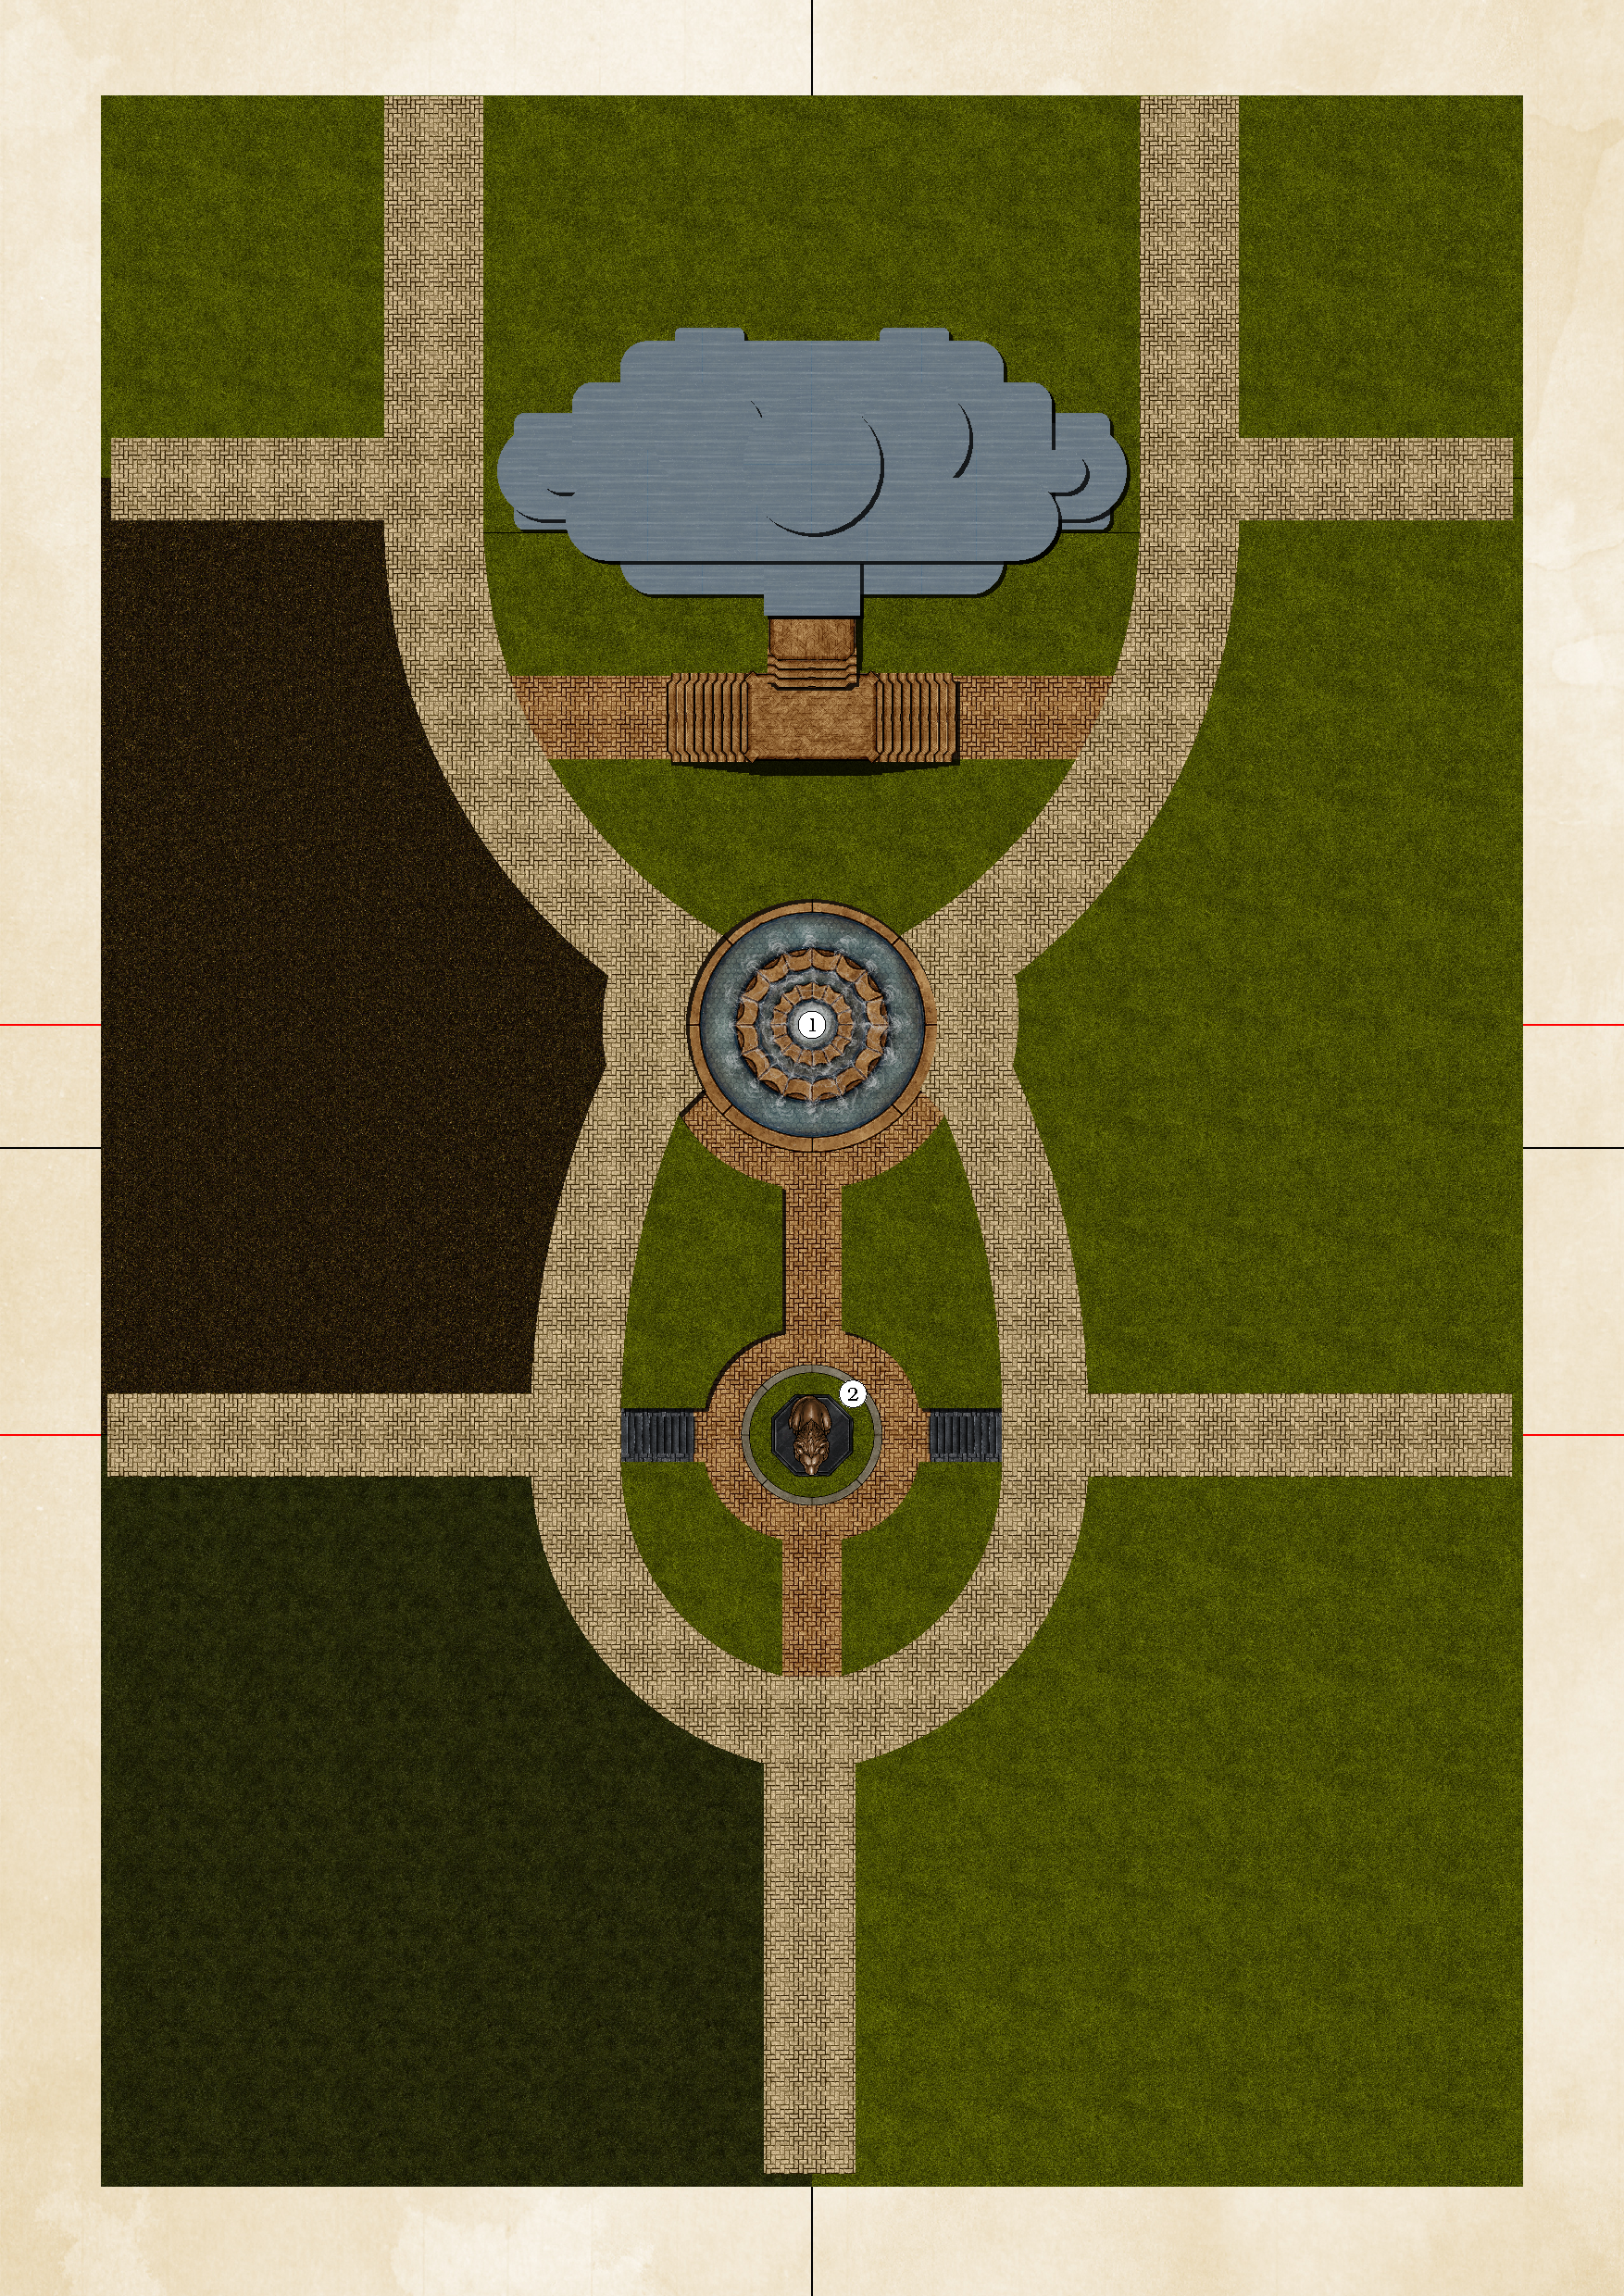
\includegraphics[width=1.2\linewidth, align=top]{\PATH adventures/Penguins_of_Madagascar/operation_Smile_and_Wave/images/Botanical_Garden.jpg}\vspace{.5em}\linebreak%
					{\fontsize{12}{12}\selectfont{%
						The meticulously landscaped grounds invite guests on a journey through different climates and habitats, from the humid tropics to arid deserts, each area presenting its unique collection of plants. Special attention has been given to the presentation and preservation of these botanical wonders, with state-of-the-art facilities ensuring their health and longevity.
						
						One of the garden's standout features is the "Ominous Beauty" exhibit, which showcases plants that are as beautiful as they are rare and dangerous. This includes the newly named "Spiranthes Vexum," a plant with a captivating swirl of red and purple at its heart, drawing crowds eager to glimpse its unique beauty.
						
						Educational programs and interactive tours are planned to enrich visitors' experiences, offering insights into the importance of plant conservation and the role botanical gardens play in environmental stewardship.
						
						The garden is not only a place of beauty and learning but also a critical step towards the city’s commitment to sustainability and biodiversity.
									
					\hfill\linebreak}}%
					&%
					{\fontsize{12}{12}\selectfont{%
						Spiranthes Vexum
						
						The opening of Central Park's Botanical Garden introduced the public to Spiranthes Vexum, a plant with mesmerizing red and purple swirls. Its extraordinary resilience and pest resistance, while impressive, have sparked concerns among experts about its potential to become invasive.
						
						Dr. Helena Morris, the garden's curator, highlights its adaptability, and opportunities that research would bring with it.
						
						Botanist Dr. Alexei Petrov underscores the need for caution, pointing out the balance between admiration for its beauty and awareness of its potential danger.
						
						\hfill\linebreak
						\vspace{-0.6\fontdimen6\font}\hspace*{-0.1\linewidth}\includegraphics[width=1.2\linewidth, align=top]{\PATH adventures/Penguins_of_Madagascar/operation_Smile_and_Wave/images/Spiranthes_Vexum.jpg}\vspace{.5em}\linebreak%
					
					\hfill\linebreak}}%
				\end{tabular}%
			}%
		\end{tikzpicture}%
	};
\end{tikzpicture}
\clearpage
\section*{Newspaper (Half-Deciphered)}
\phantomsection\addcontentsline{toc}{section}{Newspaper (Half-Deciphered)}\label{sec:HalfDecipheredNewspaper}
\begin{tikzpicture}[inner sep=0pt, remember picture, overlay]
	\node[yshift=-1em] at (current page.center) {%
		\begin{tikzpicture}
			\newspaper{\dimexpr\linewidth - 25 pt\relax}{39}{new}{%
				New York Times~~~~
			}{%
				Monday\\Sports p.4\\Weather p.31\\
			}{%
				Business  --  Politics  --  Editorial  --  Obituaries  --  TV and Radio  --  City Life
			}{%
				\setlength{\tabcolsep}{14pt}%
				\begin{tabular}{p{0.205\linewidth}p{0.41\linewidth}p{0.205\linewidth}}%
					\multicolumn{3}{c}{{\fontsize{28}{28}\selectfont{\newspaperHeaderFont Central Park Botanical Garden Opens Its Gates\linebreak}}}\\
					{\fontsize{12}{12}\selectfont{%
						\textbf{New York, NY -} Central Park's newest attraction, a sprawling Botanical Garden, officially opened its gates to the public this weekend, unveiling a collection of the world's most exotic and newly discovered plants. The grand opening event, marked by vibrant ceremonies and attended by city officials, plant enthusiasts, and curious locals, has already been hailed as a landmark addition to New York City's green spaces.
						
						The garden, designed to be a sanctuary within the bustling city, features an array of rare flora collected from the farthest reaches of the globe. Among the highlights are species that have never before been seen by the public, sparking interest and excitement among researchers and nature lovers alike.
						
						\textit{“We are thrilled to introduce visitors to the wonders of our planet’s biodiversity,” said Dr. Helena Morris, the garden's head curator. “Each plant tells a story, and with some species being showcased for the first time, we're opening chapters of nature’s book that were previously unread.”}
					
					\hfill\linebreak}}%
					&%
					\vspace{-0.6\fontdimen6\font}\hspace*{-0.1\linewidth}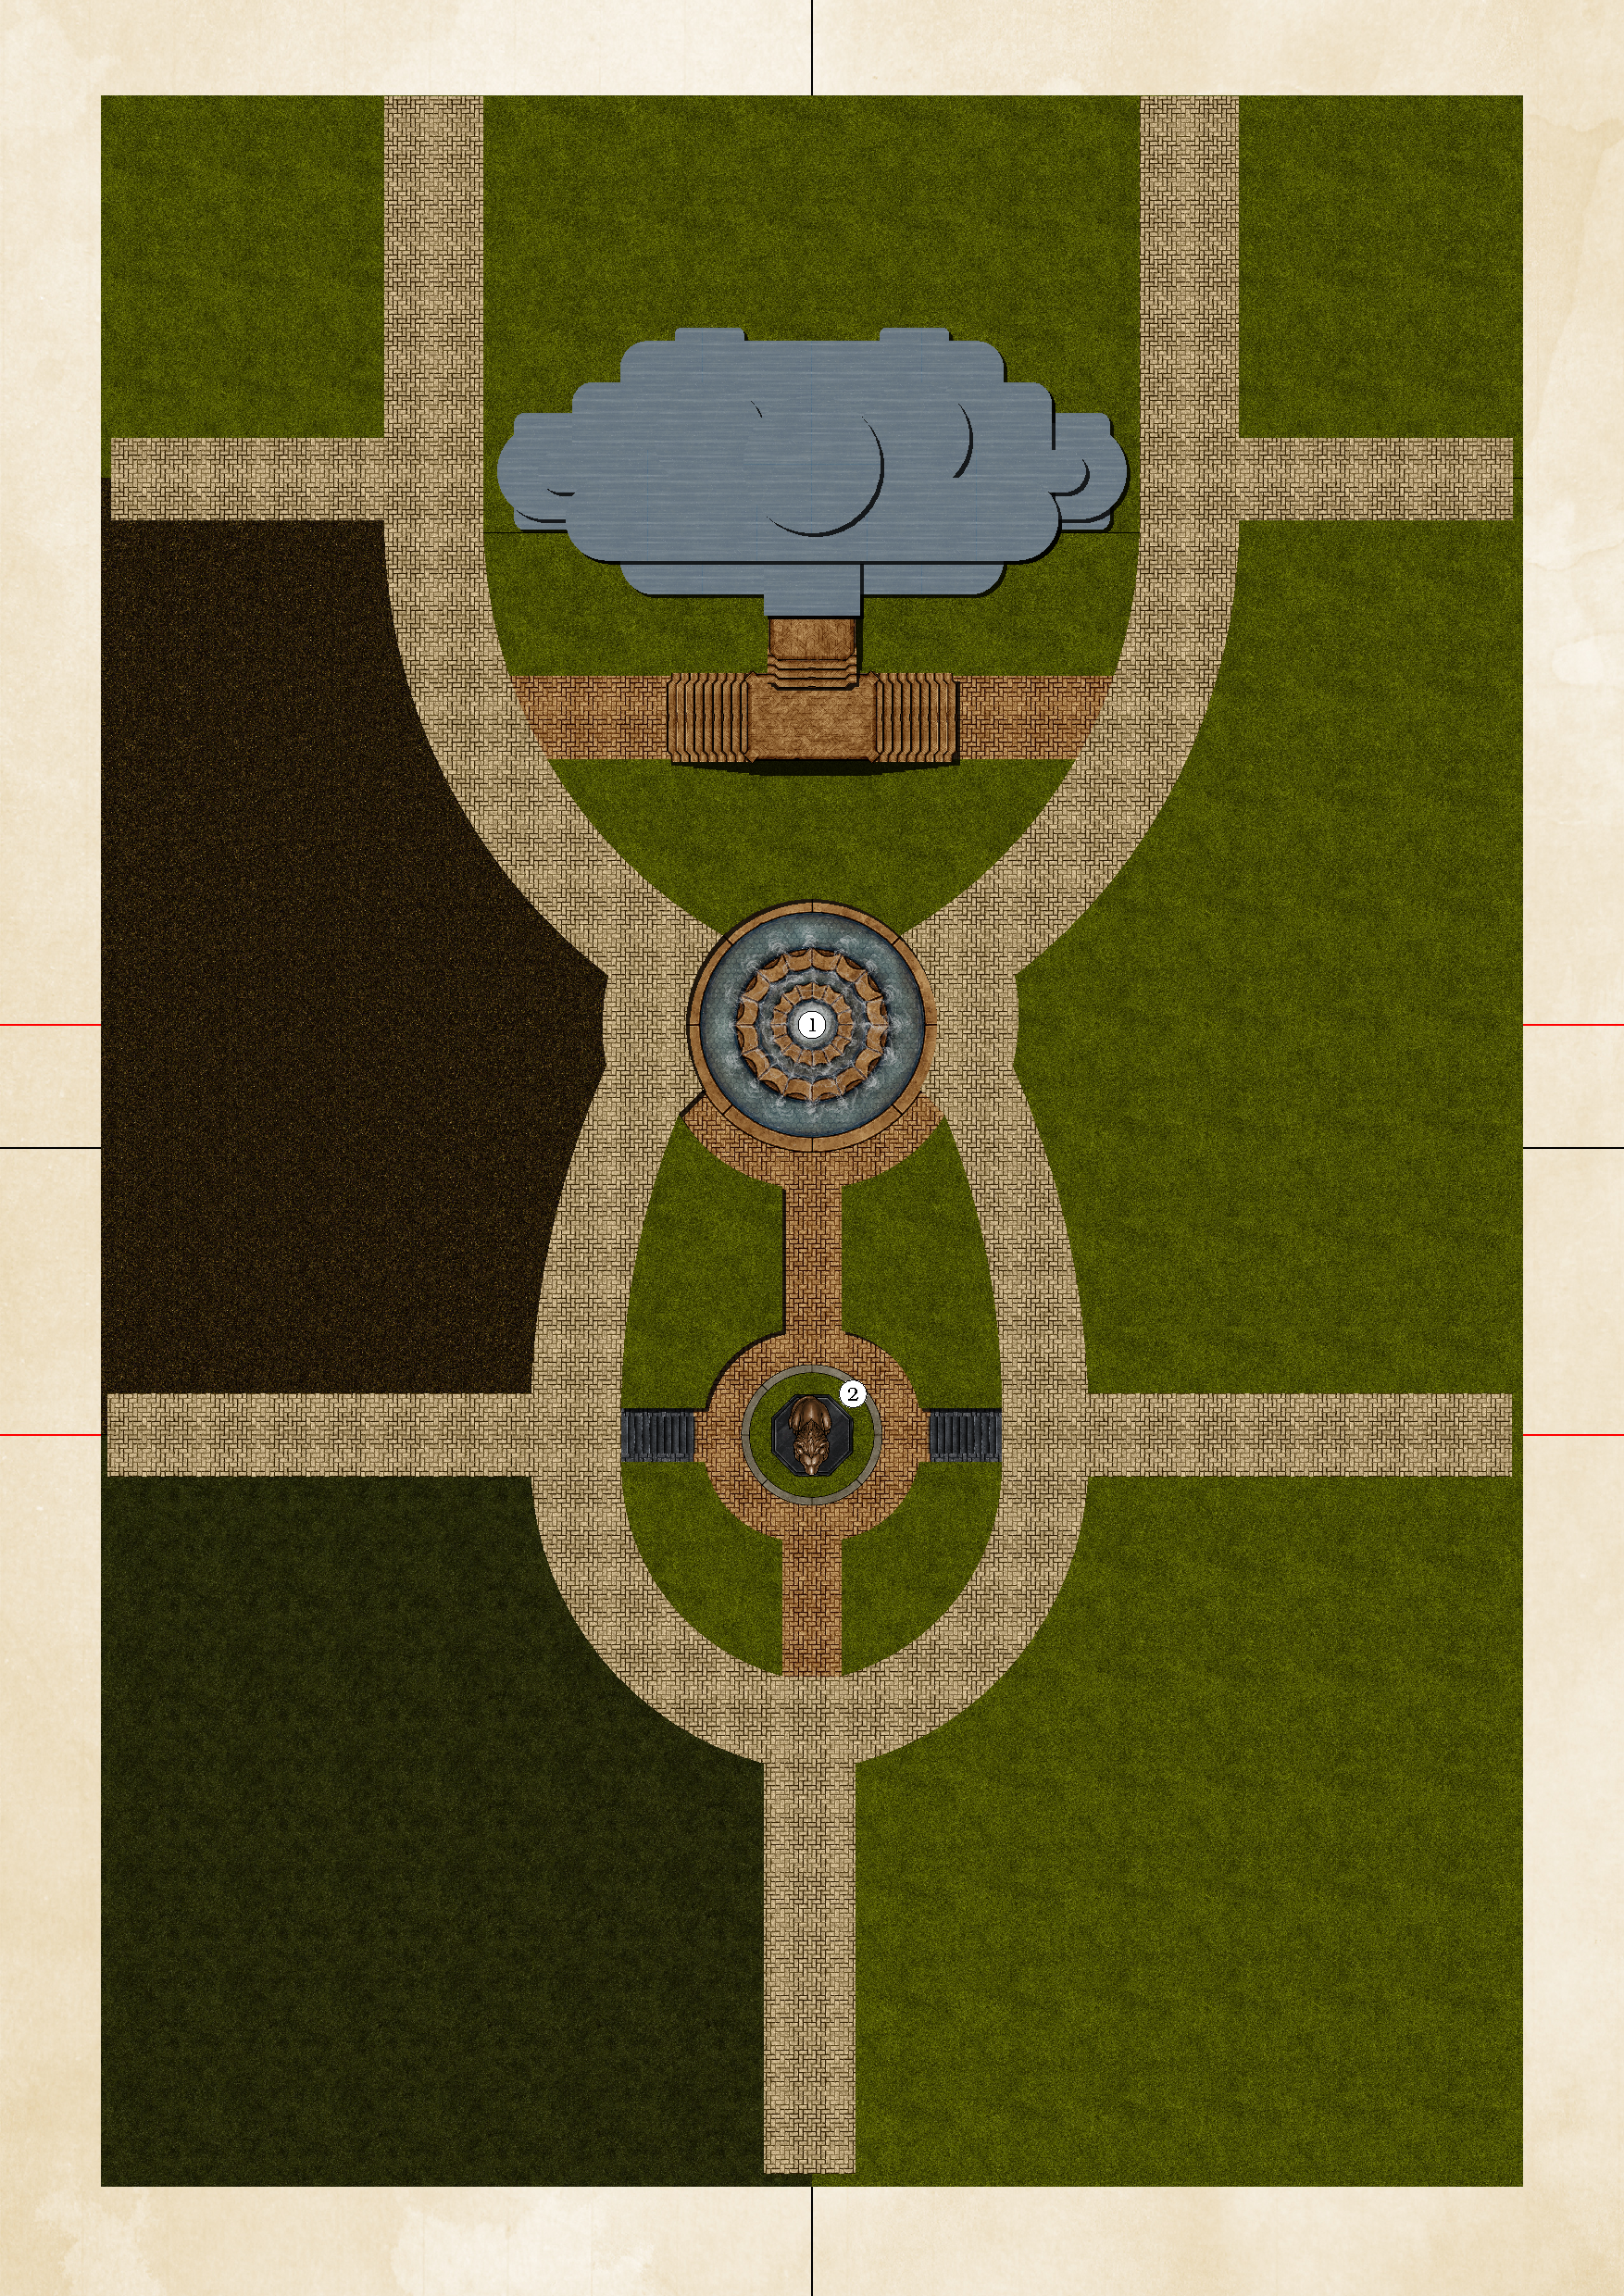
\includegraphics[width=1.2\linewidth, align=top]{\PATH adventures/Penguins_of_Madagascar/operation_Smile_and_Wave/images/Botanical_Garden.jpg}\vspace{.5em}\linebreak%
					{\fontsize{12}{12}\selectfont{%
						The meticulously landscaped grounds invite guests on a journey through different climates and habitats, from the humid tropics to arid deserts, each area presenting its unique collection of plants. Special attention has been given to the presentation and preservation of these botanical wonders, with state-of-the-art facilities ensuring their health and longevity.
						
						One of the garden's standout features is the "Ominous Beauty" exhibit, which showcases plants that are as beautiful as they are rare and dangerous. This includes the newly named "Spiranthes Vexum," a plant with a captivating swirl of red and purple at its heart, drawing crowds eager to glimpse its unique beauty.
						
						Educational programs and interactive tours are planned to enrich visitors' experiences, offering insights into the importance of plant conservation and the role botanical gardens play in environmental stewardship.
						
						The garden is not only a place of beauty and learning but also a critical step towards the city’s commitment to sustainability and biodiversity. “By bringing these plants to the heart of New York, we hope to inspire a deeper appreciation for the natural world and its preservation,” Morris concluded.
						
						With its doors now open, the Botanical Garden offers a serene escape to nature lovers and an educational adventure to those looking to learn more about the planet's diverse flora. The garden promises to be a cherished addition to Central Park, contributing to New York City’s reputation as a vibrant, ever-evolving metropolis.
									
					\hfill\linebreak}}%
					&%
					{\cipherfont\fontsize{12}{12}\selectfont{%
						\textbf{Spiranthes Vexum}
								
						The opening of Central Park's Botanical Garden introduced the public to Spiranthes Vexum, a plant with mesmerizing red and purple swirls. Its extraordinary resilience and pest resistance, while impressive, have sparked concerns among experts about its potential to become invasive.
						
						Dr. Helena Morris, the garden's curator, highlights its adaptability, and opportunities that research would bring with it.
						
						Botanist Dr. Alexei Petrov underscores the need for caution, pointing out the balance between admiration for its beauty and awareness of its potential danger.
						
						\hfill\linebreak
						\vspace{-0.6\fontdimen6\font}\hspace*{-0.1\linewidth}\includegraphics[width=1.2\linewidth, align=top]{\PATH adventures/Penguins_of_Madagascar/operation_Smile_and_Wave/images/Spiranthes_Vexum.jpg}\vspace{.5em}\linebreak%
					
					\vspace{-1.2\fontdimen6\font}\hfill\linebreak}}%
				\end{tabular}%
			}%
		\end{tikzpicture}
	};
\end{tikzpicture}
\clearpage
\section*{Newspaper (Deciphered)}
\phantomsection\addcontentsline{toc}{section}{Newspaper (Deciphered)}\label{sec:DecipheredNewspaper}
\begin{tikzpicture}[inner sep=0pt, remember picture, overlay]
	\node[yshift=-1em] at (current page.center) {%
		\begin{tikzpicture}
			\newspaper{\dimexpr\linewidth - 25 pt\relax}{39}{new}{%
				New York Times~~~~
			}{%
				Monday\\Sports p.4\\Weather p.31\\
			}{%
				Business  --  Politics  --  Editorial  --  Obituaries  --  TV and Radio  --  City Life
			}{%
				\setlength{\tabcolsep}{14pt}%
				\begin{tabular}{p{0.205\linewidth}p{0.41\linewidth}p{0.205\linewidth}}%
					\multicolumn{3}{c}{{\fontsize{28}{28}\selectfont{\newspaperHeaderFont Central Park Botanical Garden Opens Its Gates\linebreak}}}\\
					{\fontsize{12}{12}\selectfont{%
						\textbf{New York, NY -} Central Park's newest attraction, a sprawling Botanical Garden, officially opened its gates to the public this weekend, unveiling a collection of the world's most exotic and newly discovered plants. The grand opening event, marked by vibrant ceremonies and attended by city officials, plant enthusiasts, and curious locals, has already been hailed as a landmark addition to New York City's green spaces.
						
						The garden, designed to be a sanctuary within the bustling city, features an array of rare flora collected from the farthest reaches of the globe. Among the highlights are species that have never before been seen by the public, sparking interest and excitement among researchers and nature lovers alike.
						
						\textit{“We are thrilled to introduce visitors to the wonders of our planet’s biodiversity,” said Dr. Helena Morris, the garden's head curator. “Each plant tells a story, and with some species being showcased for the first time, we're opening chapters of nature’s book that were previously unread.”}
					
					\hfill\linebreak}}%
					&%
					\vspace{-0.6\fontdimen6\font}\hspace*{-0.1\linewidth}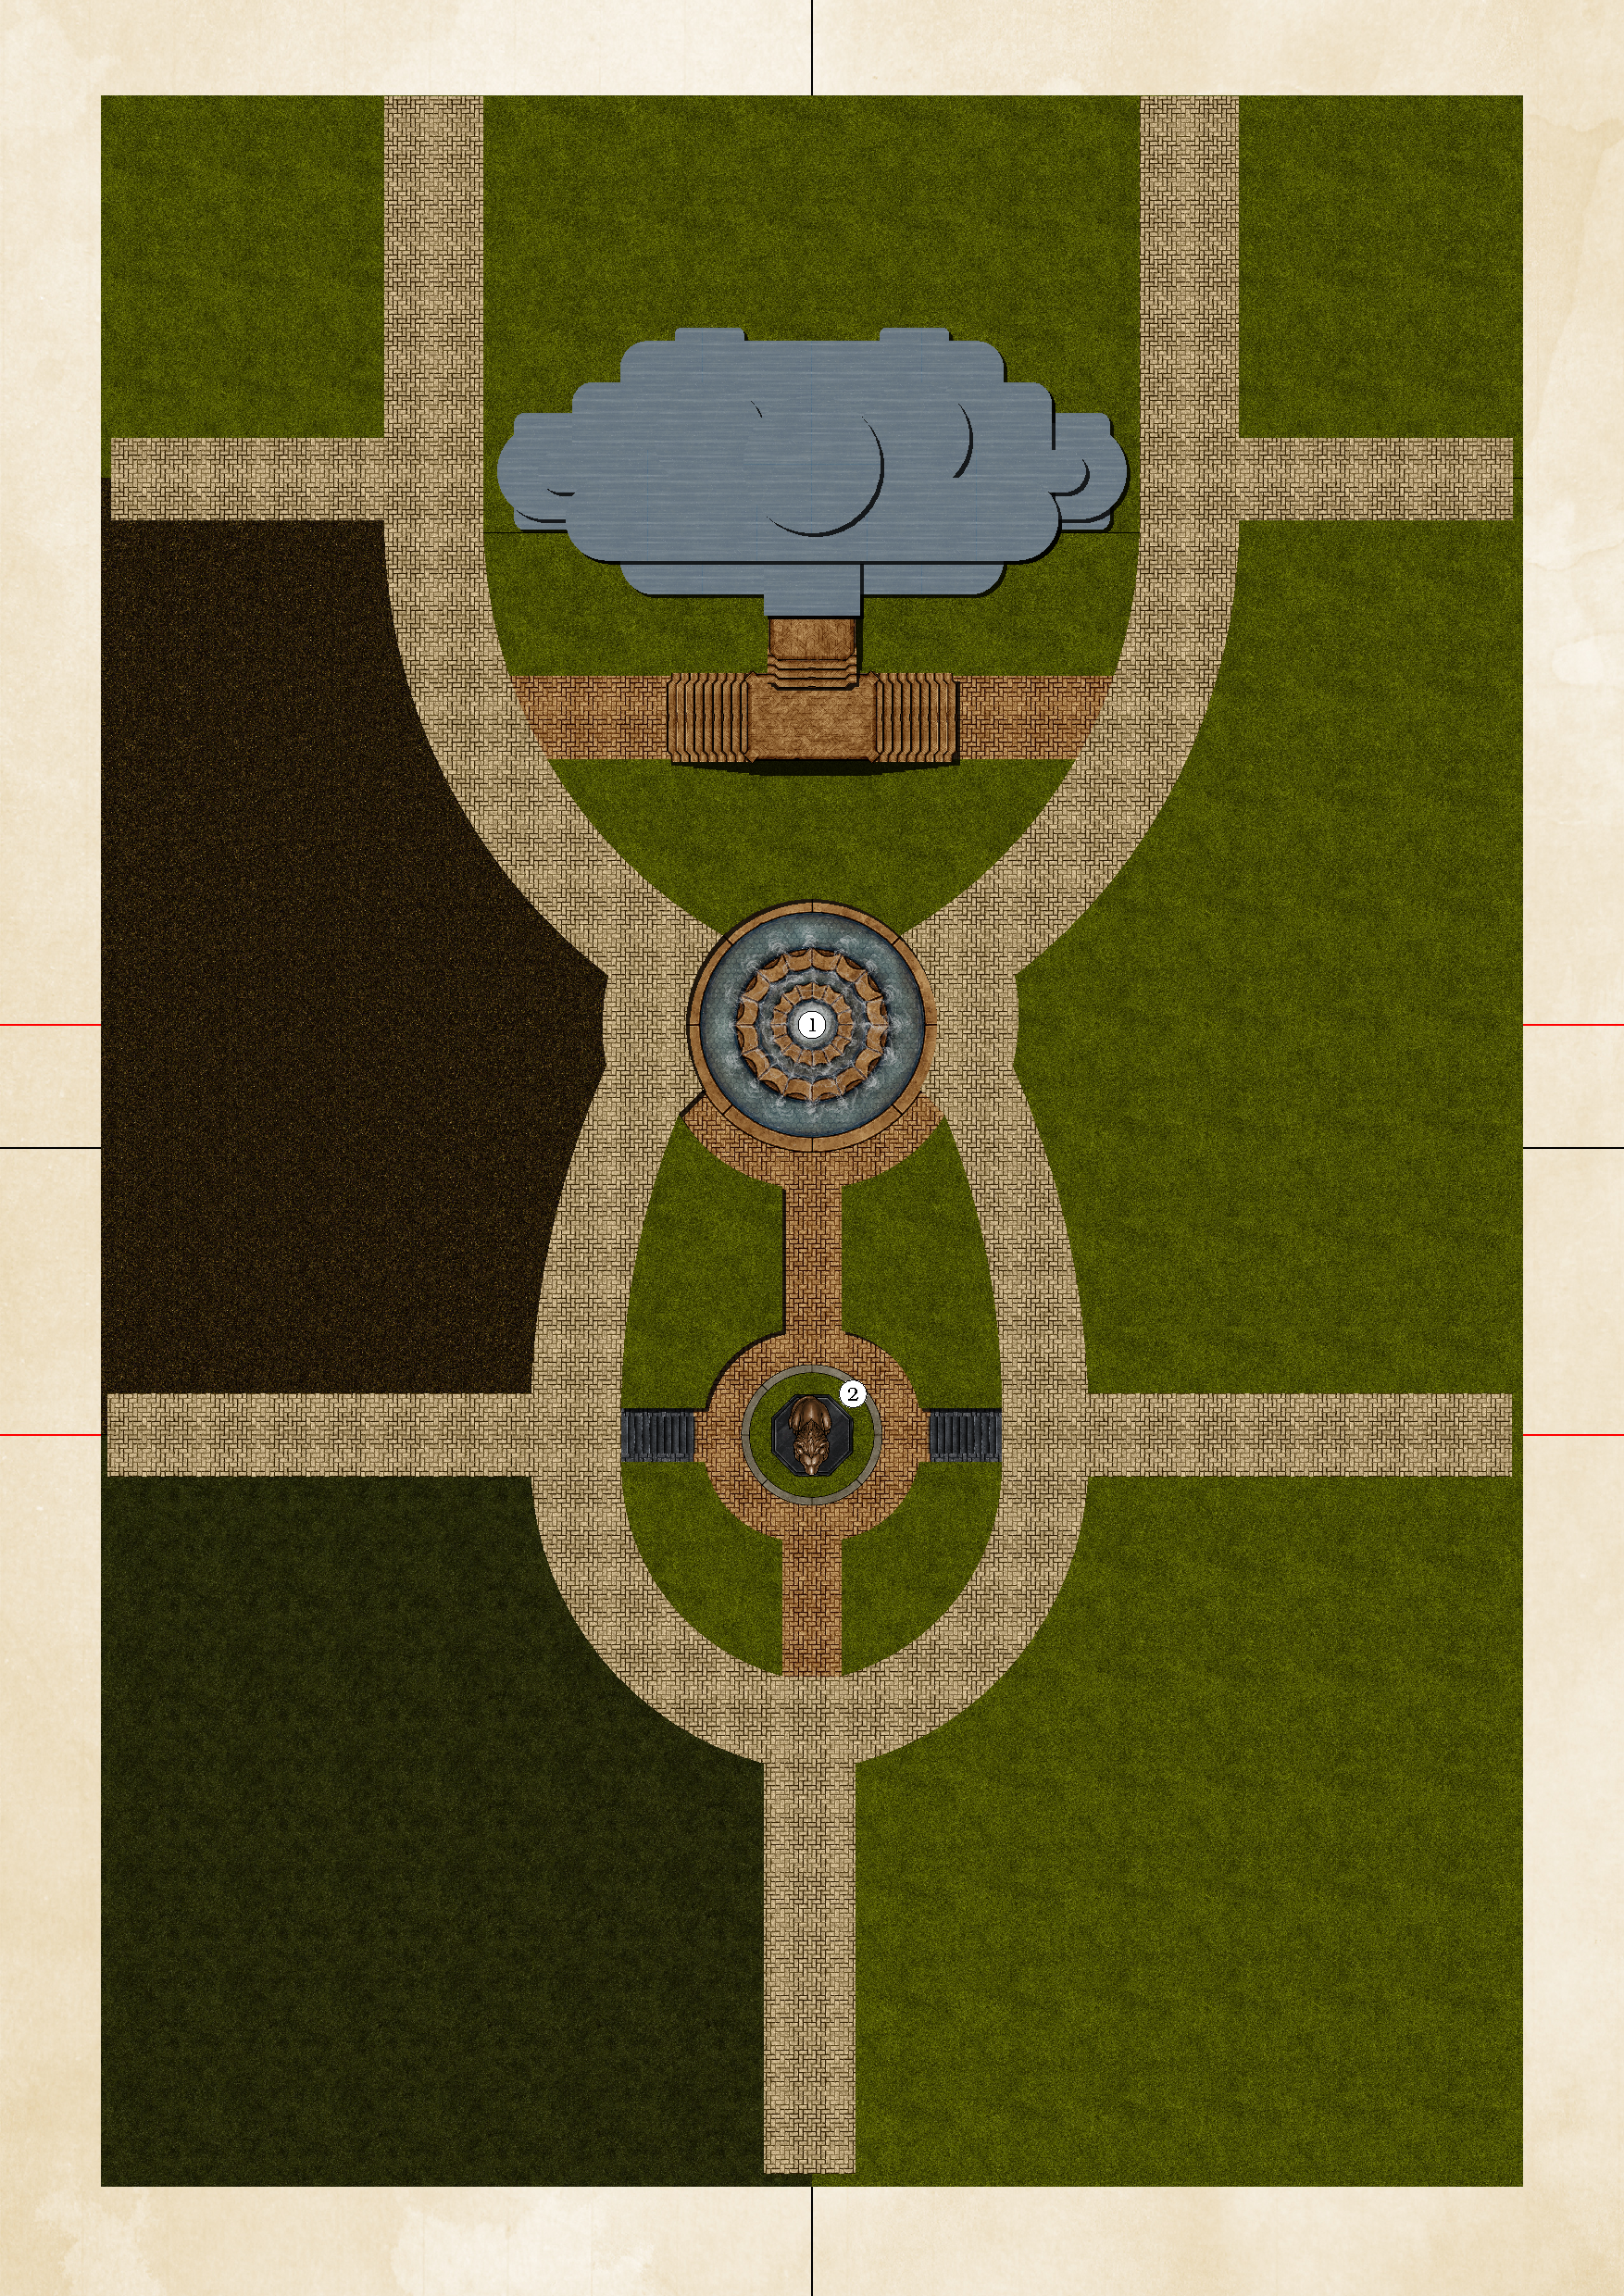
\includegraphics[width=1.2\linewidth, align=top]{\PATH adventures/Penguins_of_Madagascar/operation_Smile_and_Wave/images/Botanical_Garden.jpg}\vspace{.5em}\linebreak%
					{\fontsize{12}{12}\selectfont{%
						The meticulously landscaped grounds invite guests on a journey through different climates and habitats, from the humid tropics to arid deserts, each area presenting its unique collection of plants. Special attention has been given to the presentation and preservation of these botanical wonders, with state-of-the-art facilities ensuring their health and longevity.
						
						One of the garden's standout features is the "Ominous Beauty" exhibit, which showcases plants that are as beautiful as they are rare and dangerous. This includes the newly named "Spiranthes Vexum," a plant with a captivating swirl of red and purple at its heart, drawing crowds eager to glimpse its unique beauty.
						
						Educational programs and interactive tours are planned to enrich visitors' experiences, offering insights into the importance of plant conservation and the role botanical gardens play in environmental stewardship.
						
						The garden is not only a place of beauty and learning but also a critical step towards the city’s commitment to sustainability and biodiversity. “By bringing these plants to the heart of New York, we hope to inspire a deeper appreciation for the natural world and its preservation,” Morris concluded.
						
						With its doors now open, the Botanical Garden offers a serene escape to nature lovers and an educational adventure to those looking to learn more about the planet's diverse flora. The garden promises to be a cherished addition to Central Park, contributing to New York City’s reputation as a vibrant, ever-evolving metropolis.
									
					\hfill\linebreak}}%
					&%
					{\fontsize{12}{12}\selectfont{%
						\textbf{Spiranthes Vexum}
								
						The opening of Central Park's Botanical Garden introduced the public to Spiranthes Vexum, a plant with mesmerizing red and purple swirls. Its extraordinary resilience and pest resistance, while impressive, have sparked concerns among experts about its potential to become invasive.
						
						Dr. Helena Morris, the garden's curator, highlights its adaptability, and opportunities that research would bring with it.
						
						Botanist Dr. Alexei Petrov underscores the need for caution, pointing out the balance between admiration for its beauty and awareness of its potential danger. As Spiranthes Vexum draws visitors, it also prompts reflection on the unforeseen consequences of introducing such a powerful species into another ecosystem.
						
						\hfill\linebreak
						\vspace{-0.6\fontdimen6\font}\hspace*{-0.1\linewidth}\includegraphics[width=1.2\linewidth, align=top]{\PATH adventures/Penguins_of_Madagascar/operation_Smile_and_Wave/images/Spiranthes_Vexum.jpg}\vspace{.5em}\linebreak%
					
					\vspace{-1.2\fontdimen6\font}\hfill\linebreak}}%
				\end{tabular}%
			}%
		\end{tikzpicture}
	};
\end{tikzpicture}
\twocolumn
\renewcommand{\boolCharacterSheetImage}{true}\clearpage%
\phantomsection\addcontentsline{toc}{chapter}{Characters}\addcontentsline{toc}{section}{Kowalski}%
\CharacterSheetInput[spellcasting=true]{adventures/Penguins_of_Madagascar/characters/level_3/Kowalski/Kowalski}%
\clearpage%
\phantomsection\addcontentsline{toc}{section}{Private}\CharacterSheetInput[spellcasting=true]{adventures/Penguins_of_Madagascar/characters/level_3/Private/Private}
\clearpage
\section*{Optional: Private Mystery}\phantomsection\addcontentsline{toc}{section}{Optional: Private Mystery}
\subsection*{Private's Character Development (Ideas)}
\begin{itemize}
	\item \textbf{Hexblade Curse}\\
	When Private misses an attack on a creature within 30ft of him, he will curse at the target that he missed, using some even for him unknown language. When the creature dies he will feel invigorated as he gains HP (level + Charisma Modifier - minimum of 1). Therefore, Private realizes that he can curse his target.
	\item \textbf{Hex Warrior}\\
	When Private uses a martial or simple weapon that does not have the two-handed property and does damage to any creature, he realizes that it does much more damage than it usually would.
	\item \textbf{Investment of the Chain Master}\\
	As soon as Private finds a familiar he realizes that it has additional features
	\item \textbf{Pact of the Chain}\\
	As soon as Private finds a familiar he realizes that it has additional features
	\item \textbf{Spell Sniper}
	If Private hits 5 consecutive spell attacks or a creature that is hiding in half or three-quarter cover, he will wonder why his accuracy is greatly improved learning that he is a Spell Sniper.
	\item \textbf{Spells}
	As a Warlock Private can cast different spells. However, as he is not aware of those he will realize, most often just by chance, that he can use those, either by certain circumstances or by different opportunities in the game world.
	\begin{itemize}
		\item \textcolor{titlered}{\textbf{Mage Hand}}\\
		During the random quest encounter at the lake in the Central Park, Private will save a gosling by casting Mage Hand.
		\item \textcolor{titlered}{\textbf{Armor of Agathys (Glacial Wall)}}\\
		When Private is stuck in the powdered snow in the polar bear habitat for more than one turn, and successfully frees himself from this predicament he realizes that some snow particles are floating around him, forming a kind of shield or aura. This effect gives Private 5 Temporary HP and each creature that attacks him with a melee attack takes 5 cold damage. After this situation Private gains the ability to cast "Glacial Wall", which is indifferent from the effect of "Armor of Agathys".
		\item \textcolor{titlered}{\textbf{Hex (Weakening)}}\\
		When one creature is successful on three ability saving throw checks within one round of combat, Private lashes out with unknown incantations, cursing the target. With this he successfully casts Hex with the targeted ability to be the last ability save that the creature was able to resolve.\\
		A creature under the influence of this spell also takes additional 1d6 necrotic damage whenever it is hit by an attack made by Private.\\
		When the target dies the curse can be switched to another creature within range as a Bonus Action.
		\item \textcolor{titlered}{\textbf{Find Familiar}}\\
		After unlocking the food storage a small animal will approach the group of adventurers asking for food. If the animal is given food it will offer to become the loyal familiar of private, such Private gins the ability to cast Find Familiar.
		\item \textcolor{titlered}{\textbf{Darkness}}\\
		Private can learn this spell when the Dark Forest puzzle is solved.
		\item \textcolor{titlered}{\textbf{Invisibility}}\\
		Private can learn this spell from the chameleon in the Reptile House.
	\end{itemize}
\end{itemize}
\clearpage%
\phantomsection\addcontentsline{toc}{section}{Blank Private}%
\CharacterSheetInput[spellcasting=true]{adventures/Penguins_of_Madagascar/characters/level_3/blank_Private/blank_Private}%
\clearpage%
\phantomsection\addcontentsline{toc}{section}{Rico}%
\CharacterSheetInput{adventures/Penguins_of_Madagascar/characters/level_3/Rico/Rico}%
\clearpage%
\phantomsection\addcontentsline{toc}{section}{Skipper}%
\CharacterSheetInput{adventures/Penguins_of_Madagascar/characters/level_3/Skipper/Skipper}%
\clearpage%
\phantomsection\addcontentsline{toc}{section}{King Julien}%
\CharacterSheetInput[spellcasting=true]{adventures/Penguins_of_Madagascar/characters/level_3/King_Julien/King_Julien}%
\clearpage%
\phantomsection\addcontentsline{toc}{section}{Maurice}%
\CharacterSheetInput[spellcasting=true]{adventures/Penguins_of_Madagascar/characters/level_3/Maurice/Maurice}%
